\documentclass[a4paper 12pt]{article}
\usepackage[margin=1in]{geometry}
\usepackage{natbib}
\usepackage{epsfig}
\usepackage{amsmath}
\usepackage{amsfonts}
\usepackage{float}
\usepackage{rotating} 
\usepackage{caption}
\usepackage{subfig}
\usepackage{booktabs}
\usepackage{adjustbox}
\usepackage[table]{xcolor}
\usepackage{tabularx}
\usepackage{caption}
\usepackage{enumerate}
\usepackage{enumitem}
\captionsetup{font=footnotesize}
\newcommand{\ra}[1]{\renewcommand{\arraystretch}{#1}}
\textheight 9.0 in
\textwidth 6.5 in
\topmargin -0.5 in
\oddsidemargin 0.0in
\renewcommand{\topfraction}{1}
\renewcommand{\bottomfraction}{1}
\renewcommand{\textfraction}{0}
\renewcommand{\floatpagefraction}{0.90}
\definecolor{TableEven}{rgb}{0.8000,0.9216,0.9490}
\usepackage{makecell}
%\usepackage{fourier} 
\numberwithin{equation}{section}
\usepackage{array}
\usepackage{titlesec}
\usepackage{sectsty}
\sectionfont{\centering}
\setcounter{secnumdepth}{4}
\usepackage{natbib}
\usepackage{siunitx}
\usepackage[toc,page]{appendix}
\usepackage{sectsty}
\usepackage{scalerel,stackengine}
\stackMath
\usepackage{graphicx}
%\titleformat{\subsection}    
%       {\normalfont\fontfamily{phv}\fontsize{12}{17}\bfseries\itshape}{\thesubsection}{1em}{}
\subsectionfont{\normalfont\bfseries\itshape}
\subsubsectionfont{\normalfont\itshape}
%\usepackage[colorlinks,citecolor=DeepPink4,linkcolor=DarkRed, urlcolor=DarkBlue]{hyperref}
%\usepackage[svgnames]{xcolor} 
%
%\usepackage[colorlinks]{hyperref}
%\hypersetup{citecolor=DeepPink4}
%\hypersetup{linkcolor=DarkRed}
%\hypersetup{urlcolor=DarkBlue}
%\usepackage{cleveref}

%hyperlink for website will need a better option. highlights all equations etc
 \usepackage{hyperref}


\renewcommand{\baselinestretch} {2.0}
\makeatletter
\setcounter{page}{1}
\def\doublespace{\def\baselinestretch{1}\@normalsize}
\def\enddoublespace{}
\title{\bf 
}   
% \footnotemark}
\author{}
\date{}
\@addtoreset{equation}{section}
\renewcommand{\sp}{\vspace{0.2 in}}
\renewcommand{\theequation} {\arabic{section}.\arabic{equation}}
%\renewcommand{\thefigure}{\arabic{section}.\arabic{figure}}
\renewcommand{\thefootnote}{\fnsymbol{footnote}}
\newtheorem{theorem}{Theorem}
\newtheorem{lemma}{Lemma}[section]
\newtheorem{remark}{Remark}[section]
\newtheorem{corollary}{Corollary}[section]
\newtheorem{exam}{Example}[section]
\newtheorem{proposition}{Proposition}[section]

\newcommand{\Bigskip}{\vspace{0.3 in}}

\usepackage{xspace}
\newcommand{\m}{\textnormal{\sffamily m}\xspace}
\newcommand{\cm}{\textnormal{\sffamily cm}\xspace}
\newcommand{\g}{\textnormal{\sffamily g}\xspace}
\newcommand{\kg}{\textnormal{\sffamily kg}\xspace}


\makeatletter
\let\latex@xfloat=\@xfloat
\def\@xfloat #1[#2]{%
  \latex@xfloat #1[#2]%
  \def\baselinestretch{1}
  \@normalsize\normalsize
  \normalsize
}
\makeatother

\newcommand\longitude[1]{\directlua{ longitude ( \luastring{#1} ) }}


\usepackage{lineno}
\linenumbers

 
\begin{document}
\title{An analysis of the North Sea International Bottom Trawl Survey Data}

\maketitle


\begin{abstract}
In this research we present non-parametric estimation procedures for calculating abundance at age indices, and investigate the sensitivity of these estimates with respect to the number of otholits collected at sea. The procedures presented are applied to the North Sea International Bottom Trawls Survey data for cod (\textit{Gadus morhua}) and saithe (\textit{Pollachius virens}). We demonstrate how much information would be lost if the survey design was defined such that fewer otholits were collected. The abundance at age indices introduced differ from non-parametric indices provided by IBTS by how the age given length relation (ALK) is included. We use ALK's without the assumption of constant ALK over pre defined areas. All abundance at age indices are presented with variance estimates. Currently, such variance estimates are \textit{only} utilized for assessment of Herring (\textit{Clupea harengus}) in the North Sea, even thou they may include valuable information from the survey.

%The North Sea International Bottom Trawl Survey (IBTS) was started by the International Centre for the  Exploration of the Sea (ICES) in 1990. Seven research vessels using standardized fishing methods participates in the survey. The survey with these vessels, which allows fishing also on rough ground provides information on seasonal distribution of stocks and abundance,  which forms the basis for stock assessments. Estimates of abundance indices based on age-length keys (ALK) are provided without any assessment of their accuracy.  We present a model-based ALK estimator, and a stratified design-based ALK estimator for estimating abundance at age. Both estimators take into the spatial differences in age-length structures. These estimators are compared with the designed-based ALK estimator proposed by ICES for IBTS, which does not account for spatial differences in the age-length structure. As the proposed ALK estimator by ICES is a combination of age data over a large area, this can result in biased estimates of numbers-at-age. An example of cod (\emph{Gadus morhua}) in ICES subareas IVa and IVb is used to illustrate spatial differences in the proportions of age-at-length, and estimates of uncertainty are presented using nonparametric bootstrapping. In general, the model-based ALK estimator provides a more accurate coverage probabilities compared with the other estimators.  
\end{abstract}


\section{Introduction}
Fish stock assessments are used by fishery managers for making management decisions regarding catch quotas. The assessments provide fundamental information about the status of the stock, for instance, whether the stock is increasing and support for increased levels of harvest should be given, or whether the stock is decreasing and stricter control on harvest should be implemented. Associated with the parameters used in fish stock assessment is their uncertainty, which should not be ignored when formulating management policies \citep{walters1981effects, ludwig1981measurement}. This uncertainty can arise from many sources including natural variability, estimation procedures and lack of knowledge regarding the parameter \citep{ehrhardt1997role}. The North Sea International Bottom Trawl Survey (IBTS) data, coordinated by the International Council for the Exploration of the Sea (ICES), provides information on seasonal distribution of stocks and estimates of abundance indices and catch in numbers of fish per age-class without an assessment of the accuracy of these estimates.  As pointed out by  \citet{ludwig1981measurement} estimates of parameters relating to stock size are of little value unless they are accompanied by uncertainty estimates. The indices of abundance at age from IBTS  are based on data obtained from a stratified semi-random sampling approach of trawl stations,  and  it is essential to account for the sampling approach so as to produce reliable variance estimates \citep{lehtonen2004practical}. If the sampling approach is ignored, the effect on the variance  of the parameters could be substantial.  In particular, the variance could be greatly inflated  due to the clustering effect, which involves intra-cluster correlation of the variables \citep{aanes2015efficient, lehtonen2004practical}. 

There are two separate {\bf cost full aspects?} of the North Sea International Bottom Trawl Survey (IBTS) for generating abundance indices per age.  The first consist of calculating indices per \textit{length} class, which are obtained by trawling in a predefined {\bf procedure?} and counting the number of fish caught. Then that knowledge is transformed to indices with respect to age. The latter part is achieved with an age-length key (ALK), which is constructed by sampling otoliths in a stratified procedure from each haul and/or sub-area. To our best knowledge, there has been no research on how much the uncertainty of the abundance indices is related to these two distinct parts. The main contribution of this article is to shed light on how the indices estimates and their associated uncertainty estimates change if less effort was spent on collection of otoliths. We achieve the reduction of otoliths by mimicking a defined sampling procedure with less effort. We also focus on the spatial distribution of the ALK, and such spatial structures in the ALK has also been investigated in \citet{berg2012spatial, hirst2012bayesian}.

Currently, abundance indices from IBTS are reported in DATRAS \citep{datras} using an age-length key (ALK) \citep{fridriksson1934calculation} which is assumed to be constant over relatively large areas. In this paper we propose two ALKs which accounts for spatial variation: i) a nonparametric  haul based ALK, and ii) a spatial model-based ALK. These ALKs are described in section \ref{sec:methods}, and the results from the model based ALK gives a strong case for assuming variation in the ALK within RFAs. %In section \ref{sec:modelBasedALK} we introduce a spatial model based ALK, and see figure \ref{fig:40cmCod2015} for an illustration of spatial variation in the ALK. 
A spatial model based ALK \citep{berg2012spatial} is currently used for assessment in the North Sea with use of IBTS data. The model introduced in \citet{berg2012spatial} is similar to the model used in this paper; the main difference is that we include the spatial structure through a spatial random field \citep{lindgren2011explicit} and not through two dimensional splines \citep{wood2017generalized}.%(see Figure \ref{fig:40cmCod2015}, which shows the estimated age probabilities of a 40 cm cod (\emph{Gadhus morhua}) in the first quarter of 2015). Figure \ref{fig:40cmCod2015} shows that the age distribution clearly varies for a 40 cm cod within Central North Sea and Northern North Sea (see second graph in the first panel). 
 An  overview of the  North Sea International Bottom Trawl Survey is given in Section \ref{overview}. The current estimators for ALK and catch per unit effort (CPUE) used by ICES in their database for trawl surveys (DATRAS) and our proposed ALK estimators are given in Section \ref{sec:methods}. Two case studies, in which the methods described in Section \ref{sec:methods} are applied to, are given in Section \ref{sec:data}, and a discussion is given in Section \ref{sec:discussion}.% The results are given in Section \ref{sec:results} and a discussion is given in Section \ref{sec:discussion}.



\subsection{Overview of the North Sea International Bottom Trawl Surveys}
\label{overview}
\indent The North Sea International Bottom Trawl Survey was formed in 1991, which is a combination of the International Young Herring Survey (IYHS) and eight national surveys in the North Sea, Skagerrak and Kattegat areas. These surveys began in the 1960's, and the 1970's and 1980's, respectively. The IYHS was developed with the aim of obtaining annual recruitment indices for the combined North Sea herring \emph{Clupea harengus} stock \citep{ICES2012}, but yielded valuable information on other fish species such as cod \emph{Gadus morhua} and haddock \emph{Melanogrammus aeglefinus}.\\
\indent The North Sea IBTS began with quarterly surveys providing information on seasonal distribution of stocks sampled, hydrography and the environment, which allows changes in fish stock to be monitored and abundance of all fish species (Table \ref{fishspecies}) to be determined. These quarterly surveys, however became difficult to sustain as countries experienced budget cuts making it impossible to maintain high levels of research vessel effort. As such, in 1997 countries carried out a survey only twice a year; a first quarter survey (January-February) and a third quarter survey (August-September). The target species of IBTS fished from 1991-2018 includes standard pelagic species: Herring (Clupea harengus), Sprat (Sprattus sprattus) and Mackerel (Scomber scombrus); and standard roundfish species: Cod (Gadus morhua), Haddock (Melanogrammus aeglefinus), Saithe (Pollachius virens),  Norway Pout (Trisopterus esmarkii)  and Whiting (Merlangius merlangus).

% Table \ref{fishspecies} gives the common names (scientific names in parentheses) of the target species that are sampled during the quarterly North Sea International Bottom Trawl Surveys. The common names of the species in parentheses will be used in the rest of paper.\\
%\clearpage
%\begin{small}
%\begin{table}[h!]
%\centering
%\setlength\tabcolsep{1.5pt} 
%\captionsetup{font=small, width = 8.5cm}{
%\caption{Species fished in the NS-IBTS from 1991-2017.}\label{fishspecies}}
%\begin{tabular}{cccccccccc}
%\hline \\
%\multicolumn{2}{c}{} \\
%Standard Pelagic               & Standard Roundfish & By-Catch Gadoid       \\[1.5ex]
%\hline \\[0.1ex]
%Herring (Clupea harengus) &  Cod (Gadus morhua)  & Pollock (Pollachius)      \\[1.5ex]
%Sprat (Sprattus sprattus)   &Haddock (Melanogrammus aeglefinus) & Pouting (Trisopterus luscus) \\[1.5ex]
%Mackerel (Scomber scombrus) & Norway Pout (Trisopterus esmarkii) & Trisopterus minutus (Poor Cod) \\[1.5ex]
% & Saithe (Pollachius virens)  & Blue Whiting (Micromesistius poutassou)   \\[1.5ex]
%&Whiting (Merlangius merlangus)  & Hake (Merluccius merluccius)  \\[1.5ex]
%& &  Ling (Molva molva) \\[1.5ex]
%& &  Tusk (Brosme brosme) \\[0.5ex]
%\hline
%\end{tabular}
%\end{table}
%\end{small}
Research vessels from seven nations in the first quarter (Q1) and six nations in the third quarter (Q3) are used for conducting surveys on all finfish species in the North Sea during January-February and July-August, respectively, between 1997-2017 (Table \ref{countries} in Web appendix \ref{secAp:areasfishedappendix} gives details of the different research vessels). The sampling frame is defined by the ICES index or roundfish areas (RFA) as shown in Figure \ref{icesroufismap} numbered 1 to 10, and which we refer to as superstrata \citep{nottestad2015quantifying, fuller2011sampling}. These  roundfish areas were substratified into small strata defined by non-overlapping statistical rectangles of roughly $30 \times 30$ nautical miles ($1^{o} \  \mathrm{Longitude} \ \times  \  0.5^{o} \ \mathrm{Latitude}$), and were convenient to use for North Sea IBTS as they were already being used for fisheries management purposes. Most statistical rectangles contain a number of possible tows that are deemed free of obstructions, and vessels are free to choose any position in the rectangles as long as the hauls are separated by at least 10 nautical miles within and between rectangles. However, all countries select tows based on a semi-random approach from datababes of national safe tows or DATRAS or commercial fishing data, except Sweden who uses fixed stations and in some cases depth-stratified semi-random sampling design \citep{ICES2018}, and England who also uses fixed stations and only conduct surveys during the third quarter. In some rectangles, sampling may be further stratified due to significant changes in seabed depth which may, in turn, cause variations in the fish population. In particular, the North Sea IBTS herring, saithe and sprat data are weighted by depth strata in the statistical rectangle (see Table \ref{tab:weights} in appendix \ref{secAp:weightings}). It is also a requirement that countries avoid clustering their stations between adjacent rectangles in order to reduce positive serial correlation, and thereby maximize survey precision.  The latest major reallocation of rectangles occurred in 1991, but since then the survey has tried to keep at least one vessel in every subarea in which it had fished in the most recent years. Minor reallocation of rectangles between Norway, Scotland and Germany was done in 2013. Each rectangle was  typically sampled twice by two different countries before 1997, but after that target coverage of two trawl hauls per rectangle per survey  was introduced because of national financial constraints \citep{ICES2015}. But in some rectangles in the Eastern English Channel, Southern North Sea and Central North Sea intensified sampling is carried out.\\
\indent The recommended standard trawling gear of the North Sea IBTS is the mulitpurpose chalut {\`a} Grande Ouverture Verticale (GOV) trawl \citep{ICES2012}, which has been used on all participating vessels since 1992, while different pelagic and bottom trawls suitable for fishing finfish species were used before 1992. Standardized trawling protocols were adopted with a towing speed of 4 knots but depending on vessel performance, tide and weather conditions the average towing speed can be at minimum 3.5 and maximum 4.5 knots. From 2000-2018 trawling is done during the daylight hours, which are considered 15 minutes before sunrise to 15 minutes  after sunset \citep{ICES2012}. After each trawl the total catch of the different species is weighed on board and biological parameters such as length for all fish species caught (to 0.1$\cm$ below for shellfish, to 0.5$\cm$ below for herring and sprat and to 1$\cm$ below for all other species) are collected. Where the numbers of individuals are too large for all of them  to be measured to obtain the length distribution, a representative subsample of 100 fish is selected. Otoliths are collected on board from a small fraction of all the target species from all  round fish areas (RFAs) (Figure \ref{icesroufismap}) to retrieve age reading. Table \ref{tab:otolithsTable} in Web appendix \ref{secAp:otolithappendix} gives the minimum sampling levels of otoliths for the target species.
%\indent The trawl tow locations are selected using a  semi-random approach with at least two primary sampling units (PSU) per stratum, where PSUs are standardized swept-area trawl hauls. Sampling locations for all countries are proposed in advance in order to increase the randomisation of sampling. These locations are based on a random selection on a random selection of valid tows with start and end position executed in the period 2000-2017. In the unusual event that no ``clear" tow exists the cruise leader, who select the haul positions, may select to undertake a ``blind" tow on unknown ground after checking the proposed trawl track for hazardous seadbed obstructions with acoustic methods. \\

\begin{figure}[h!]
  \centering
 {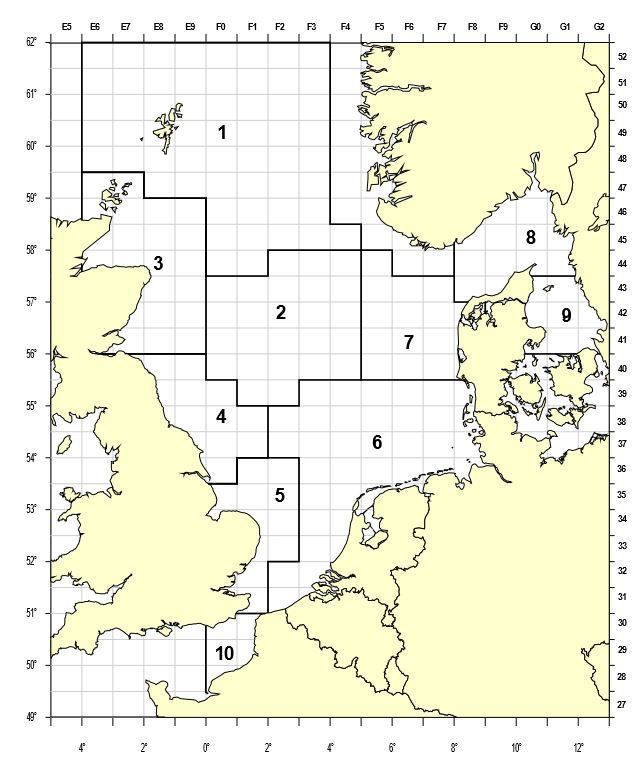
\includegraphics[width=10.5cm]{icesroundfishmap.jpg}}   
 \captionsetup{font= footnotesize, width=13cm}{
 \caption{Standard roundfish areas used for roundfish since 1980, for all standard species since 1991. Additional RFA 10 added in 2009. For example, the number 1 indicates ICES Index Area 1, and an ICES Statitical rectangle (ST) in IA 1 is 43F1 \citep{ICES2015}.}\label{icesroufismap}}
\end{figure}

\section{\large METHODS}
\label{sec:methods}
This section gives the estimators of abundance indices. The estimators are haul time-based and utilizes an ALK approach. We consider the ALK approach used in DATRAS and we propose two ALK estimators. The ALK used in DATRAS for computing abundance indices does not account explicitly for the spatial distribution in the age-length composition, which may be different and would result in a biased ALK. This difference may be caused either by variation in length-at-age distributions or by variations in the relative abundance of age classes, that is age-at-length distributions \citep{gerritsen2006simple}.  To account for the spatial distribution we propose a design-based ALK estimator that is haul dependent (Section \ref{sec:haulestimator}) and a model-based ALK estimator (\ref{sec:spatialModelALK}).
\subsection{Catch per unit effort}
\label{sec:cpueestimators}
In this paper, the catch per unit effort (CPUE) is defined as the number of fish of a certain species and age or length which are caught per hour trawl. In this section we define the CPUE matematically, which explains how the index is calculated. 

For a given species of interest, let $n_{h,l}$ be the number of fish with length $l$ caught by trawl haul $h$. The CPUE for a given length $l$ by trawl haul $h$ is defined as 
\begin{equation}\label{eq:cpueHaul}
\mathrm{CPUE}_{h,l} =\frac{n_{h,l}}{d_h},
\end{equation}
were $d_h$ is the duration of the trawl in hours. The CPUE per age class is further defined as
\begin{equation}\label{eq:cpueALK}
\mathrm{CPUE}_{h,a} =\sum_{l \in {\bf L}}\mathrm{CPUE}_{h, l} \times ALK_{a,l,h},
\end{equation}
where ${\bf L}$ is the set of all length classes and $ALK_{a,l,h}$ is the age length key, which represents the estimated proportion of fish with age $a$ in $l$th length class in haul $h$. For a given number of trawl hauls in a statistical rectangle, the mean CPUE defined as  mCPUE  in a statistical rectangle can be expressed as the average CPUE of the trawl hauls in the statistical rectangle:
\begin{equation}\label{eq:cpueRec}
\mathrm{mCPUE}_{s,a} =\sum_{h \in H_{s}}\frac{\mathrm{CPUE}_{h,a}}{|H_{s}|}.
\end{equation}
Here $H_{s}$ represents the set of trawl hauls taken in statistical rectangle $s$, and $|H_{s}|$ is the number of hauls taken in the rectangle. The mCPUE in $p$th RFA is further defined as
\begin{equation}\label{eq:cpueRFA}
\mathrm{mCPUE}_{p,a} = \sum_{s \in S_{p}} \frac{\mathrm{mCPUE}_{s,a}}{|S_{p}|} \omega_s,
\end{equation}
where $S_{p}$ is the set of all statistical rectangles in RFA $p$, $|S_{p}|$ is the number of statistical rectangles in RFA $p$, and $\omega_s$ is a weight variable for each statistical rectangle. The weight variable $\omega_s$ varies between species. For some species $\omega$ equals 1 (e.g. Gadus morhua) for all $s$, and for other species it is the proportion of the statistical rectangle which has depth between 10 to 200 meters, for example Pollachius virens (see Table \ref{tab:weights} in Web appendix \ref{secAp:weightings}  for weightings of statistical rectangles).  The index for abundance at age in the whole study area, $mCPUE_{N,a} $, is further defined by
\begin{equation}
mCPUE_{N,a} = \frac{\sum_{p\in {\bf P}} A_{p}  \mathrm{mCPUE}_{p,a}}{A_{\text{total}}}.
\label{abundanceestimatornorthsea}
\end{equation}
Here ${\bf P}$ is the set of RFAs, $A_p$ is the area of RFA $p$, and $A_{\text{total}} = \sum_{p\in {\bf P}} A_{p}$.

 

\subsection{ALK Estimators}

The definition of the CPUE of age includes an ALK, see (\ref{eq:cpueALK}), which we described in this section. Three ALK estimators are included in this paper, which are named as follows:  \textit{i}) DATRAS ALK, \textit{ii}) haul based ALK and \textit{iii}) model based ALK.
% In this section we define these three ALK estimators. 
\subsubsection{DATRAS ALK}
\label{sec:datrasalkestimator}
Let $\text{ALK}^{\text{D}}$ denote the DATRAS ALK. The $\text{ALK}^{\text{D}}$ is defined as constant within each RFA, and is calculated for each RFA by aggregating the age observation from each RFA. $ALK^{\text{D}}_{a,l,h}$ used in equation (\ref{eq:cpueALK}) is defined as the proportion of observed fish with age $a$ in length class $l$ in the RFA $h$. If there are no observed fish in length class $l$ in the RFA, ages from length classes close to $l$ is used. The details of the procedure for borrowing strength from neighbouring length classes are given in Web appendix \ref{secAp:DATRASBorrow}. The underlying assumption of this ALK  is that age-length compositions are homogeneous within the RFAs. This is a rather strong assumption, and any violation would have an unknown impact on the estimates of abundance indices. \citet{aanes2015efficient} illustrated that violation of the assumption of constant ALK leads to biased estimates of CPUEs. 

\subsubsection{Haul based ALK}
\label{sec:haulestimator}
We define a haul dependent ALK  by  $ALK^{H}$. The $ALK^{H}_{a,l,h}$ is defined as the average proportion of observed fish with age $a$ in {\bf a pooled length class $l$ in haul $h$?}. If there are no observed ages of fish in a length class $l$ in the haul, ages from the same length class in the haul close by is used (Web appendix \ref{secAp:oursBorrow} describes the procedure in detail).

\subsubsection{Spatial Model-Based ALK Estimator}
\label{sec:spatialModelALK}
In this section we introduce a spatial model based ALK. Using such a model enables us to obtain smooth structures in the distribution of age given length. It further enables us to utilize spatial latent effects. Spatial model-based approach of age-lengths are widely used \citep{berg2012spatial, hirst2012bayesian, rindorf2001analyses}, and are used for stock assessment in the North Sea \citep{berg2014evaluation}. \\ % kvist2000using olav: double check this when i have access.
\indent Let the response variable of the age group of a fish be $a = M,...,A$ where $M$ is the youngest age, and $A$ is the oldest age which is typically defined as a "plus group". Suppose $y(l,{\bf s},h)$ is the age  of a fish with length $l$ caught at location ${\bf s}$. As in \citet{berg2012spatial} we use a continuous ratio model for the spatial age given length model. {\bf That is, let
\begin{align}\label{eq:linearPred1}
\pi_a(y(l,{\bf s})) = P(y = a|y \geq a, l, {\bf s}) = \frac{p_a(l,{\bf s})}{p_a(l,{\bf s}) + \cdots p_{A-1}(l,{\bf s})} \vspace{ 4mm} \ \ \ \text{for } a =M,...,A-1 ,
\end{align}
were $p_a(l,s)$ is the probability of a fish with length $l$ at location ${\bf s}$ to be of age $a$. Further is
\begin{align}\label{eq:linearPred}
\text{logit}\pi_a(y(l,{\bf s},h)) = \beta_a +  f_a(l) + \gamma_a({\bf s}).
\end{align}
Here $\beta_a$ is an intercept, $ f_a(l)$ is a continuous function of length and $\pmb{\gamma}$ is a mean zero Gaussian spatial random field with Mat\'{e}rn covariance function. The spatial random field is intended to capture any spatial variation in the ALK.} \\
\emph{these equations and definitions are not quite clear. these definitions of the equations need restructuring i think. we need to explain what is on the left hand side of (2.6), for example, Let the probability of a fish of age $a$ given length $l$ at location $s$ be defined as ....I do not understand the meaning of the word logit attached to the left side of (2.7) and a definition of the left hand side of (2.7) is needed also, again for example, Further, let the probability of......be...... Also, where in equation (2.6) is equation (2.7) used or called? Also, are we including haul effect in the model or has it been include already and our results are reflecting that, and if not should we state that it's possible to include random effects and how it can be done?}\\

The continuous function $f_a(l)$ in (\ref{eq:linearPred}) is modelled with usage of P-splines \citep{wood2017generalized}, and these spline regression coefficients are included as a Gaussian random effect. The precision matrix for the spline regression coefficients is constructed such that the variability (or wryggliness) in the spline is penalized, see \citet[page 239]{wood2017generalized} for details. The R package mgcv \citep{wood2015package} is used for extracting the precision matrix needed for the spline regression coefficients.

\indent We assume that the spatially Gaussian random field in (\ref{eq:linearPred}), $\pmb{\gamma}$, follows a stationary Mat\'{e}rn covariance structure:
\begin{equation}\label{eq:matern}
 \text{Cov}(\gamma(\mathbf{s}_1),\gamma(\mathbf{s}_2)) = \frac{\sigma^2_{\gamma}}{2^{\nu-1}\Gamma(\nu)}(\kappa_{\gamma}||\mathbf{s}_1 -\mathbf{s}_2||)^{\nu}K_{\nu}(\kappa_{\gamma}||\mathbf{s}_1-\mathbf{s}_2||),
\end{equation}
where $\sigma^2_{\gamma}$ is the marginal variance, $||\cdot||$ is the Euclidean distance measure in kilometres, $\nu$ is a smoothing parameter, $\kappa_{\gamma}$ is a spatial scale parameter and $K_{\nu}(\cdot)$ is the modified Bessel function of the second kind with $\nu = 1$. The spatial range parameter and marginal variances in the spatial fields are assumed to be equal across ages. The spatial field is estimated with the stochastic partial differential equation (SPDE) procedure described in \citet{lindgren2011explicit}. The main concept behind the SPDE procedure is that the precision matrix of a spatial field with Mat\'{e}rn  covariance function can be approximated by a sparse matrix on a grid covering the area of interest. Such a grid and sparse precision matrix are constructed with use of the R-INLA package \citep{rue2009approximate}.

The model based ALK estimate is obtained by maximizing the likelihood. We maximize the likelihood with use of an R-Package called Template Model Building ({\sffamily TMB}),  \citep{kristensen2015tmb} combined with the optimizing function {\sffamily nlminb} in R. In this application {\sffamily TMB} is advantageous as it utilizes sparse structures in the latent fields, {\bf it Laplace approximate the latent fields?}, and uses automatic derivation. A laptop with  processor intel(R) Core(TM) i5-6300 CPU @ 2,40 GHz, used approximately 2 minutes  to estimate the {\bf model.? }

\subsection{Uncertainty estimation}
\label{sec:uncertaintyestimation}
In this section we describe how the uncertainty of the CPUE estimates are calculated. We use nonparametric bootstrapping to quantify the uncertainty of the CPUEs. Nonparametric resampling allows us to estimate the sampling distribution of the CPUE empirically without making assumptions concerning the data. The percentile method is used to estimate $95\%$ confidence intervals of the estimated CPUEs \citep{carpenter2000bootstrap}. % To obtain sufficiently accurate $95\%$ bootstrap percentile confidence intervals, the number of bootstrap samples should  be on the order of 1000 or more \citep[see][]{carpenter2000bootstrap}. 

A bootstrap procedure for estimating the uncertainty of CPUEs in the North Sea is suggested in  \citet{ICES2013}. In the rest of this paper, we refer to this procedure as DATRAS bootstrap procedure. The DATRAS procedure is divided into two parts; one part which samples CPUE per length (\ref{eq:cpueHaul}), and another part which samples the ALK used in (\ref{eq:cpueALK}). The DATRAS bootstrap procedure is based on the assumption of homogeneous CPUE within RFAs. This assumption is likely to be wrong, and will typically cause an overestimation of the uncertainty. Therefore, we have included a bootstrap procedure, defined as the stratified bootstrap procedure, which instead assumes constant CPUE within each statistical rectangle. 

\subsubsection{DATRAS and stratified bootstrap procedures}
\indent In this subsection we elaborate the bootstrap procedure for catch at length proposed by \emph{DATRAS} \citep{ICES2013} and the stratified procedure, and elaborate how the ALK is simulated. Assume there are $N_{\text{s}}$ trawl hauls in a statistical rectangle. The DATRAS bootstrap procedure consists of sampling with replacement $N_{\text{s}}$ of all trawl hauls in the corresponding RFA, and place them in the statistical rectangle. This procedure is performed independently across all statistical rectangles. Recall that this procedure is based on the assumption that CPUE is homogeneous in the whole RFA. The stratified bootstrap procedure is a modification of the DATRAS bootstrap procedure. Rather than sampling hauls from the whole RFA, we  sample the $N_{\text{s}}$ trawl hauls from the list of hauls within the same statistical rectangle. If there are only one trawl hauls within an statistical rectangle, we sample either that haul or the closest haul in air distance.

For simulating the DATRAS ALK we sample with replacement age observations within each RFA stratified with respect to length. If there is only one observed age from a given length class, we sample either that age or at random one age of the closest length class with observed ages. For the haul based ALK, we use the observed ages in the sampled hauls when simulating the CPUE per length ({\bf is this from the stratified bootstrap procedure? what about explanations for the model based ALK?}).

\subsection{Reducing sampling effort}
\label{sec:optimizationsampling}
%The North sea IBTS is carried twice a year: quarter 1 (January -February) and quarter 3 (July-September). We examined the sampling effort carried out over a five year period for IBTS for both quarters. From 2013 to 2018, on average there were 368 valid trawl hauls taken over an average period of 43 ship days in the first quarter between 6 nations, and 346 valid trawl hauls taken over an average of... ship days in third quarter between 7 nations. The number of otolith sampling per species per varies per length group and by nation. Some nations, for example......have been sampling otoliths per round fish area according the ICES guidelines \citep{ICES2006} during the years 2013-2017, while other nations such as Norway, UK Scotland and Netherlands have adopted a per-haul basis of sampling otoliths (see Table \ref{tab:otolithsTable} in appendix \ref{secAp:otolithappendix}). From 2018 all nations are required to sample otoliths per specified length, for a given species, from each trawl haul. For example, for ..........1 otolith per 1 cm length class, for herring and sprat 1 otoliths per 0.5 cm length class and (haddock, whiting and Norway pout - shell fish?) 2 otoliths per 5 cm length class.  \\
%An analysis of the North Sea cod and saithe catches from the first quarter of IBTS 2015  is presented. In general, the North Sea IBTS data is registered as follows: 1) data calculated as catch in  numbers per hour trawled (denoted as C type), 2) data by haul (denoted as R type), and 3) sub-sampled data (denoted as S type). For each  species (Table \ref{fishspecies}) and by age group, abundance indices are calculated by averaging within statistical rectangles (strata) and then averaging over specific round fish areas (RFAs). Cod is typically found in all RFAs  (see Figure \ref{fig:40cmCod2015}),  but saithe is found only in specific RFAs, for example in RFA 1 (see Figure \ref{saithe2015Q1Map} in appendix \ref{secAp:saithe2015Q1Map}). In quarter 3 of 2015, the date of catch varied between 13.01.2015 to 19.02.2015, and there was a total of 387 trawl hauls. The age of cod ranged from 1 to 8 years old while for siathe the age ranged from 1 to 16 years old but catch rates are typically higher for cod (2788) compared with saithe ({\bf 492}). 
%\subsection{Summary of cod and saithe data}
The current sampling procedure for the North Sea IBTS data is the sampling of one otolith from every observed length group in every trawl (see Table \ref{tab:otolithsTable} in Web appendix \ref{secAp:otolithappendix}). We investigate the effect on the estimated mCPUE and its variance if the sampling procedure of otoliths changes such that fewer otoliths were collected. To determine this effect we remove otholits in a stratified manner, mimicking a sampling procedure where fewer otoliths are collected. For sampling fewer otoliths, we define wider length groups, for example $2$ cm, or $3$ cm, or $5$ cm and so on,  and simulate the otolith  collection such that only one otolith is sampled from every wider length group. Estimated mCPUE's with summary statistics, based on the simulated reduced data sets are then compared with the parameters estimated from using of all data. In principle, we are free to define any length class to reduce the number of observed otoliths. For simplicity we propose two procedures: i) sample at random  one otolith from every 2 cm length group, and ii) sample at random one otolith from every 5 cm length group. These are reasonable grouping procedures for the species of interest as indicated in Figure \ref{fig:codandsaithe}, since the likelihood of overlapping in these groups is small. The species and data used in this research are discussed in detail in Section \ref{sec:data}. Figure \ref{sec:codresults} gives predicted probabilities of age given length of two target species of IBTS.
\begin{itemize}
\item \emph{I thought to include this plot here to show that it's reasonable to group at 2cm and 5 cm }
\item \emph{If 2018 data would be used these plots need updating with that data}
\item \emph{include (cm) on the x-axis to demonstrate the unit used for length; write out the word "probability" on y- axis; remove bold titles on the plots}
\end{itemize}

\clearpage
\begin{figure*}[h!]
\centering
\begin{tabular}{@{}ccc@{}}
\subfloat[age-length distribution of cod]{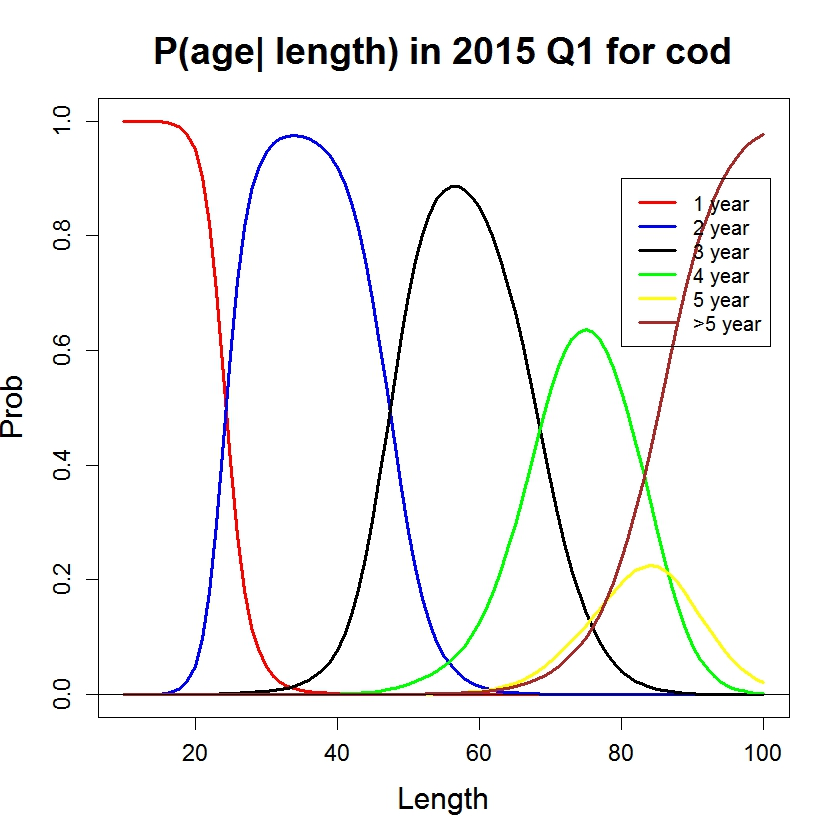
\includegraphics[width=0.45\textwidth]{cod2015Q1.jpeg}} & 
\subfloat[age-length distribution of saithe]{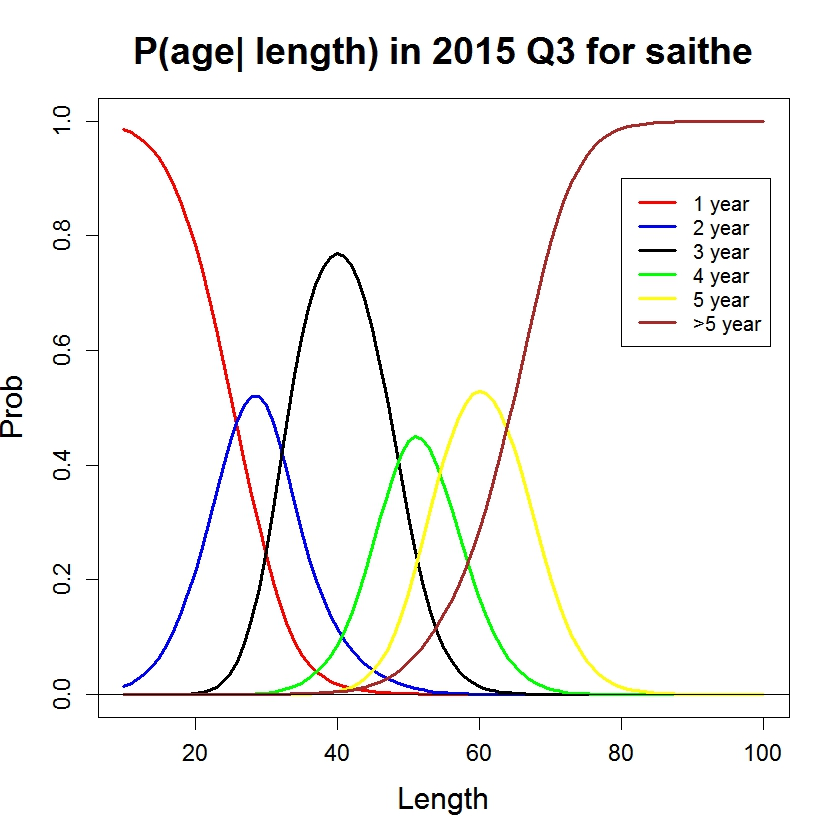
\includegraphics[width=0.45\textwidth]{saithe2015Q3.jpeg}} &
\end{tabular}
\caption[]{Predicted probabilities of age given length using the model described in (\ref{eq:linearPred1}) and (\ref{eq:linearPred}) for cod (left panel) and saithe (right panel) in Q1 and Q3, respectively in year 2015.}
\label{fig:codandsaithe}
\end{figure*} 


\section{Case studies}
\label{sec:data}
In this section we apply the methods described in Section \ref{sec:methods} to data from the International Bottom Trawl Survey for the year 2018, which is obtained from the DATRAS database \citep{datras}. We choose year 2018 because in that year new sampling procedures proposed by ICES for the collection of otoliths were introduced in the surveys. For instance, one otolith per length group is sampled for most target species (see Table \ref{tab:otolithsTable} in Web appendix \ref{secAp:otolithappendix} for details of the sampling procedures for each target species). In this paper the focal species are cod and saithe and the samples are collected in the first and third quarters. All samples are caught using the standard GOV gear described in Section \ref{overview}. Table \ref{tab:data2018} gives a brief description of the data for year 2018 in the first quarter. The data (Table \ref{tab:data2018}) shows that cod can be as old as 8 years, and saithe as old as ..... years but for simplicity, in our analyses we consider the age groups 1 to 6+ for all ALK methods, where the last group consists of fish of age 6 or older . Note that age 0 for the target species are included in IBTS and are required in the calculation of the ALKs but the results of these estimation are not included in any further analyses.

\begin{itemize}
\item \emph{logical reasons for using 2018 data but we do not have Q3 data and it was recommended by J Devine etc to use Q3 data for saithe (I am not sure of the reasons, we could clarify this) but Q1 is not recommended for saithe. Should we consider 2017 as most countries were adopting the sampling strategy of one otolith per cm at that time?}
\item \emph{possibly explain the data in Table \ref{tab:data2018} a bit more, here in this paragraph?}
\item \emph{I am unable to extract year and haul.ID from the data, subsetting etc doesnt seem to work to filter on 2018 only to fill this Table with relevant information. This is strange and I do not know why}
\end{itemize}


%\clearpage

\begin{small}
\begin{table}[h!]
\caption{Summary of North Sea IBTS cod and saithe (in parentheses) data for first quarter in year 2018.}
\begin{tabular}{llllll}
\toprule
\bf Data&\bf Description \\
\midrule
Trawl hauls  & Total of 357 trawl hauls in Q1 of 2018,   \\
&238 (83)  with length and 231 (82) with age information\\[1.3ex]
Age &The age of cod varied between 1 to 8 years, while saithe age ranged \\
& from 1 to .... \\[1.3ex]
Length & Length information in cm of each cod varied between 8 to 112 cm while saithe \\
& varied between ... to ... cm \\[1.3ex]
Date&Date of catch in Q1 varied between 13.01.2015 to 19.02.2015 and in Q3 \\
&between 26.07.2015 to 06.09.2015 \\[1.3ex]
%Statistical rectangle & The stratum in  which at least two trawl hauls are made \\[1.5ex]
%Coordinates & Geographic coordinates of each trawl haul in a statistical rectangle \\[1.3ex]
Duration of haul & Mean duration is 25.9 minutes, with 15  to 30 minutes as 90\% coverage interval. \\[1.3ex]
%Total count per age ($\mathrm{Total_{age}}$) & $3017_{1}$, $2629_{2}$, $1773_{3}$, $1051_{4}$, $460_{5}$, $194_{6}$, $58_{7}$ \\[0.5ex]
Total count for all ages & 7605 cod in Q1 of 2015 and ....saithe in Q3 of 2015. \\[0.5ex]
\bottomrule
\end{tabular}
\label{tab:data2018}
\end{table}
\end{small}

%\clearpage
\subsection{Cod and Saithe using ALK methods}
\label{sec:codresults}

Recall that the main assumption of DATRAS ALK is that the age-length compositions of species across large areas are the same. To illustrate that this assumption may not be valid, we used  the spatial ALK model to predict probabilities of age given length of a .....cm long cod and a .....cm long saithe in the North Sea (Figure \ref{predictedprobabilitiesplot}). These plots provide strong evidence against a null hypothesis of no spatial effect in the ALKs, as the likelihood of age given length changes in some areas. The plots also suggest that cod is distributed in all areas of the North Sea (Figure \ref{predictedprobabilitiesplot} (a)), whereas saithe is more likely to inhabit areas in the northern North Sea, specifically RFA 1 (Figure \ref{predictedprobabilitiesplot} (b)).

Table \ref{resultstablecodandsaithe} shows abundance indices of cod and saithe estimated from each of the three ALK methods. Estimates of abundance indices are similar 

 Both the haul based ALK and spatial ALK accounts for spatial variation in the data
%Our proposed nonparametric haul-based ALK method and spatial ALK model accounts for the spatial distribution of the ages given length 

\begin{itemize}
\item \emph{generate plots for year 2018 Q1. Possibly show same age given length group for both species?}
\item \emph{discuss differences in estimates from ALK methods (Table \ref{resultstablecodandsaithe} - in terms of relative standard error estimates; overestimation and underestimation from DATRAS (bootstrap) method not knowing the strength in either direction) - Issues:}
\begin{itemize}
\item \emph{Ignores fine scale stratification at the first stage, hence overestimation of the uncertainty}
\item \emph{Ignores age-length data collected at the haul level, hence underestimates the uncertainty}
\item \emph{Biases in both direction}
\end{itemize}
\item \emph{test for significant differences between estimates from ALK methods for age groups?}
\end{itemize}

\clearpage
\begin{figure}[h!]
\centering
\begin{minipage}[c]{0.70\linewidth}
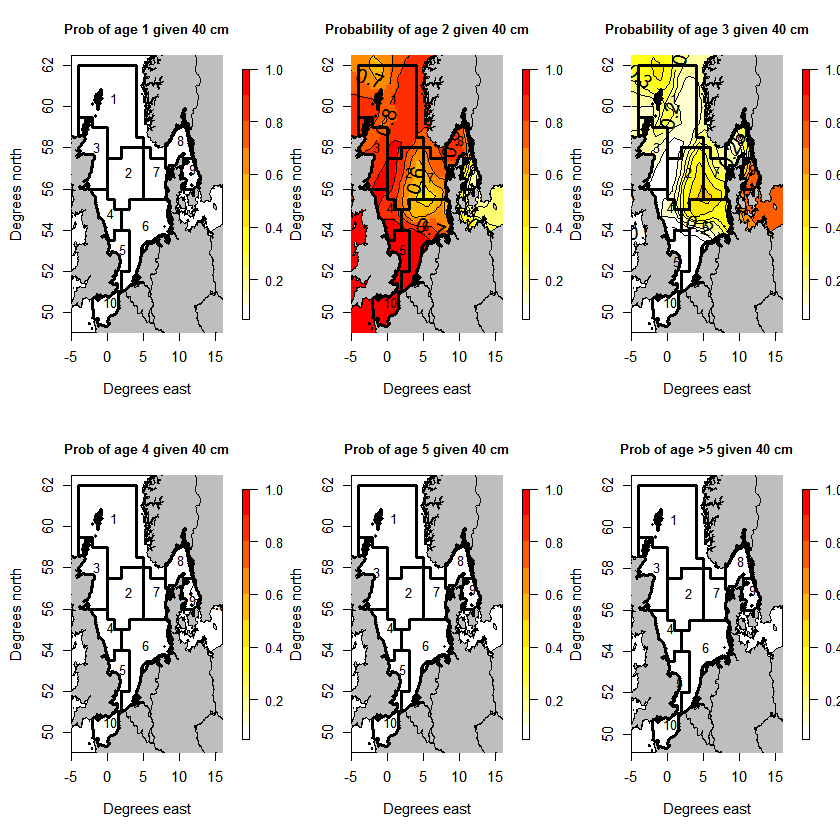
\includegraphics[width=103mm,scale=9.5]{Allcode40cm2015.png}
\caption*{\bf (a) cod}
\label{fig1.1}
\end{minipage}

\quad
\begin{minipage}[c]{0.70\linewidth}
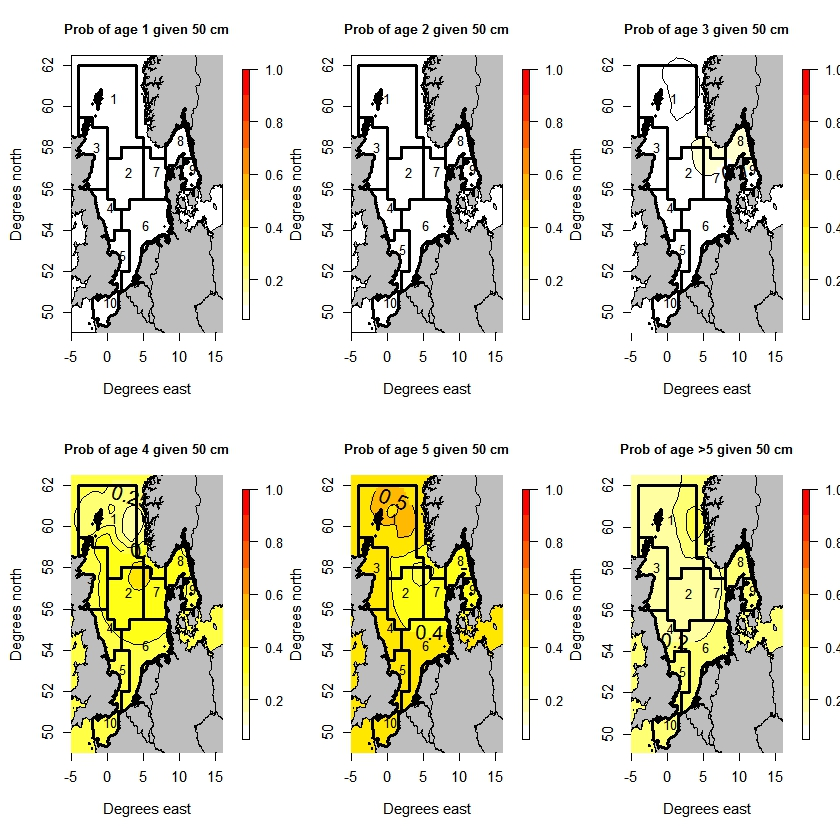
\includegraphics[width=103mm,scale=9.5]{saithe2015Q1Map.jpeg}
\caption*{\bf (b) saithe}
\label{fig5.1}
\end{minipage}
 \caption{Predicted probabilities of age given length using model (\ref{eq:linearPred1}) and (\ref{eq:linearPred}) for the year 2018 Q1. Graph (a) gives probabilities of predicted age of a ....cm long cod, and graph (b) gives probabilities of predicted age of a ....cm saithe in RFAs 1 to 10 in the North Sea.}
  \label{predictedprobabilitiesplot}
\end{figure}

%\reallywidehat{\mathbb{E}(V)}
\clearpage

\begin{tiny}
\begin{table}[h!]
\centering
\scriptsize
\setlength\tabcolsep{4.3pt} 
\captionsetup{font=small, width = 16.5cm}{
\caption{Average estimates of abundance indices for the North Sea cod and saithe species from 200 bootstrap samples and 100 simulation runs, in year 2018 Q1. Standard error estimates (SE) (relative standard error, RSE in parentheses) and the lower bounds (LB) and upper bounds (UP) of approximate $95\%$ confidence intervals from the three ALK methods are also given.}\label{resultstablecodandsaithe}}
\begin{tabular}{ccccccccccccccccccccccccccc}
\hline \\[0.1ex]
{\bf Species} &{\bf $a$ } & \multicolumn{4}{c}{\bf DATRAS ALK} & \multicolumn{4}{c}{\thead{\bf Haul-based ALK }} & \multicolumn{4}{c}{\thead{\bf  Model-based ALK}} \\[1.5ex]
 % & \multicolumn{3}{c}{DATRAS Bootstrap}   & \multicolumn{3}{c}{Stratified Bootstrap}   & \multicolumn{3}{c}{Stratified Bootstrap} \\[1.5ex]
%   \cmidrule(lr{0.5em}){2-5}  \cmidrule(lr{0.1em}){6-9} \cmidrule(lr{0.5em}){10-13}  \\ [0.1ex]
& &$\widehat{mCPUE_{N,a}}$ & SE(RSE) & LB & UB &$\widehat{mCPUE_{N,a}}$ & SE (RSE) & LB & UB   & $\widehat{mCPUE_{N,a}}$ & SE (RSE) & LB & UB &   \\[0.5ex]
\cmidrule(lr{0.5em}){3-6}  \cmidrule(lr{0.5em}){7-10}  \cmidrule(lr{0.1em}){11-14} \\ [0.1ex]
%\hline\\[1.0ex]
%\raisebox{1.5ex}{\bf cod} & 0  & 0 & 0 ( $-$) & 0 & 0 &  0   &  0 ($-$) & & & 0 & 0 ($-$)  \\[1ex]
\raisebox{1.5ex}{\bf cod}& 1  & 0.764  & 0.26 ($34 \%$) & 0.31 & 1.33 & 0.60  & 0.24 ($40 \%$) & & & 0.70 & 0.36 ($51 \%$) \\[1ex]
& 2  & 21.989 & 6.76 ($31 \%$) & 12.73 & 37.15 & 22.21 & 4.15 ($19 \%$) & & & 22.11& 4.28 ($19 \%$) \\[1ex]
& 3  & 11.285 & 2.19 ($19 \%$) & 6.31 & 15.02 & 10.58 & 1.20 ($11 \%$) & & & 10.99& 1.77 ($16 \%$) \\[1ex]
& 4  & 3.265  & 0.71 ($22 \%$) & 1.49 & 4.21 & 3.67  & 1.28 ($35 \%$) & & & 3.50 & 0.87 ($25 \%$) \\[1ex]
& 5  & 1.147  & 0.34 ($30 \%$) & 0.40 & 1.75 & 1.27  & 0.42 ($33 \%$) & & & 1.20 & 0.48 ($40 \%$) \\[1ex]
& 6+  & 1.276 & 0.38 ($30 \%$) & 0.44 & 1.82 & 1.40  & 0.70 ($50 \%$) & & & 1.21 & 0.42 ($35 \%$)\\[4.5ex]

%\raisebox{1.5ex}{\bf saithe} & 0  & 0      & 0 ( $-$)       & & & 0     &  0 ($-$)       & & & 0    & 0 ($-$)  \\[1ex]
\raisebox{1.5ex}{\bf saithe} & 1  & 0.764  & 0.26 ($34 \%$) & & & 0.60  & 0.24 ($40 \%$) & & & 0.70 & 0.36 ($51 \%$) \\[1ex]
& 2  & 21.989 & 6.76 ($31 \%$) & & & 22.21 & 4.15 ($19 \%$) & & & 22.11& 4.28 ($19 \%$) \\[1ex]
& 3  & 11.285 & 2.19 ($19 \%$) & & & 10.58 & 1.20 ($11 \%$) & & & 10.99& 1.77 ($16 \%$) \\[1ex]
& 4  & 3.265  & 0.71 ($22 \%$) & & & 3.67  & 1.28 ($35 \%$) & & & 3.50 & 0.87 ($25 \%$) \\[1ex]
& 5  & 1.147  & 0.34 ($30 \%$) & & & 1.27  & 0.42 ($33 \%$) & & & 1.20 & 0.48 ($40 \%$) \\[1ex]
& 6+  & 1.276 & 0.38 ($30 \%$) & & & 1.40  & 0.70 ($50 \%$) & & & 1.21 & 0.42 ($35 \%$)\\[0.5ex]

\hline
\end{tabular}
\end{table}
\end{tiny}


\clearpage


%
%\begin{tiny}
%\begin{table}[h!]
%\centering
%\scriptsize
%\setlength\tabcolsep{1.4pt} 
%\captionsetup{font=small, width = 16.5cm}{
%\caption{Estimates of abundance indices (Index) of saithe, and estimated standard errors for 400 bootstrap samples from DATRAS and Stratified bootstrap procedures in RFA 1 in the first quarter of year 2015. Approximate $95 \%$ confidence intervals (CI) are also given.}\label{resultstablesaithe}}
%\begin{tabular}{ccccccccccccccccccccccccccc}
%\hline \\[0.1ex]
%  & \multicolumn{3}{c}{\bf DATRAS ALK} & \multicolumn{3}{c}{\thead{\bf Haul-based ALK }} & \multicolumn{3}{c}{\thead{\bf  Model-based ALK}} \\[1.5ex]
%  & \multicolumn{3}{c}{DATRAS Bootstrap}   & \multicolumn{3}{c}{Stratified Bootstrap}   & \multicolumn{3}{c}{Stratified Bootstrap} \\[1.5ex]
%   \cmidrule(lr{0.5em}){2-4}  \cmidrule(lr{0.1em}){5-7} \cmidrule(lr{0.5em}){8-10}  \\ [0.1ex]
%{\bf Age ($a$) }  &\thead{Abundance \\ estimate} & \thead{Standard \\ error} & \thead{Relative \\ standard error} &\thead{Abundance \\ estimate} & \thead{Standard \\ error} & \thead{Relative \\ standard error} & \thead{Abundance \\ Estimate}  & \thead{Standard \\ error} & \thead{Relative \\ standard error}& \\[0.5ex]
%\cmidrule(lr{0.5em}){1-1}  \cmidrule(lr{0.5em}){2-4}  \cmidrule(lr{0.1em}){5-7} \cmidrule(lr{0.5em}){8-10}  \\ [0.1ex]
%0  & 0      & 0    & $-$  & 0    &   0   & $-$     & 0    & 0    & $-$         \\[1ex]
%1  & 0.764  & 0.26 & $34 \%$ & 0.60  & 0.24 & $40 \%$   & 0.70  & 0.36 & $51 \%$   \\[1ex]
%2  & 21.989 & 6.76 & $31 \%$ & 22.21 & 4.15 & $19 \%$   & 22.11 & 4.28 & $19 \%$   \\[1ex]
%3  & 11.285 & 2.19 & $19 \%$ & 10.58 & 1.20 & $11 \%$   & 10.99 & 1.77 & $16 \%$ \\[1ex]
%4  & 3.265  & 0.71 & $22 \%$ & 3.67  & 1.28 & $35 \%$   & 3.50  & 0.87 & $25 \%$  \\[1ex]
%5  & 1.147  & 0.34 & $30 \%$ & 1.27  & 0.42 & $33 \%$   & 1.20  & 0.48 & $40 \%$  \\[1ex]
%6+  & 1.276  & 0.38 & $30 \%$ & 1.40  & 0.70 & $50 \%$   & 1.21  & 0.42 & $35 \%$  \\[4.5ex]
%
%
% & \multicolumn{8}{c}{\bf Approximate $95 \%$ CI from bootstrap procedures} \\[1.5ex]
%0  & 0      &(0, 0)         && 0      &  (0, 0)         && 0     & (0, 0)           \\[1ex]
%1  & 0.764  &(0.31, 1.33)   && 0.60   &  (0.31, 0.91)   && 0.70  & (0.35, 1.48)    \\[1ex]
%2  & 21.898 &(12.73, 37.15) && 22.21  &  (15.64, 30.72) && 22.11 & (14.76, 30.36) \\[1ex]
%3  & 11.285 &(6.31, 15.02)  && 10.58  &  (8.74, 13.65)  && 10.99 & (8.61, 15.42)  \\[1ex]
%4  & 3.265  &(1.49, 4.21)   && 3.67   &  (2.81, 4.74)   && 3.50  &(1.96, 5.60)   \\[1ex]
%5  & 1.147  &(0.40, 1.75)   && 1.27   &  (0.67, 2.31)   && 1.20  &  (0.56, 2.78)   \\[1ex]
%6+  & 1.276  &(0.44, 1.82)   && 1.40   &  (0.78, 2.69)   && 1.21  & (0.70, 2.43)  \\[1ex]
%\hline
%\end{tabular}
%\end{table}
%\end{tiny}




\clearpage

\subsection{Optimum sampling effort for North Sea Cod and Saithe}
\label{sec:optimumeffortresults}

\begin{itemize}
\item number of otoliths taken (full data)
\item how many simulations and bootstrap samples taken
\item haul-based ALK method was used (advantages and disadvantages of using model-based)
\item how many otoliths remained after reduction (as a percentage)
\item effect of this reduction on estimate and variance 
\end{itemize}

\begin{tiny}
\begin{table}[h!]
\centering
\scriptsize
\setlength\tabcolsep{3.8pt} 
\captionsetup{font=small, width = 16cm}{
\caption{Average estimates of abundance indices and standard error estimates for the North Sea cod and saithe species when all the otolith data is used and when one otolith per 2 cm or 5 cm length group was used. The lower bounds (LB) and upper bounds (UP) of approximate $95\%$ confidence intervals from the haul-based ALK method are given.}\label{resultsoptimum}}
\begin{tabular}{ccccccccccccccccccccccccccc}
\hline \\[0.1ex]
{\bf Species} &{\bf $a$ } & \multicolumn{2}{c}{\bf Full data}  & \multicolumn{6}{c}{\thead{\bf Reduced data by $2$ cm}} & \multicolumn{6}{c}{\thead{\bf Reduced data by $5$ cm}} \\[1.5ex]
   \cmidrule(lr{0.5em}){5-10}  \cmidrule(lr{0.1em}){11-16}   \\ [0.1ex]
 && \multicolumn{2}{c}{} & \multicolumn{3}{c}{\thead{\bf $\widehat{mCPUE_{N,a}}$  }} & \multicolumn{3}{c}{$\widehat{SE}_{mCPUE_{N,a}}$ } & \multicolumn{3}{c}{\thead{\bf $\widehat{mCPUE_{N,a}}$  }} & \multicolumn{3}{c}{$\widehat{SE}_{mCPUE_{N,a}}$ } \\[1.5ex]
 % & \multicolumn{3}{c}{DATRAS Bootstrap}   & \multicolumn{3}{c}{Stratified Bootstrap}   & \multicolumn{3}{c}{Stratified Bootstrap} \\[1.5ex]

& &$\widehat{mCPUE_{N,a}}$ & $\widehat{SE}_{mCPUE_{N,a}}$   & LB  & UB & $Cv\%$   & LB &  UB & $Cv\%$ & LB  & UB & $Cv\%$   & LB &  UB & $Cv\%$ &    \\[0.5ex]
\cmidrule(lr{0.5em}){3-4}  \cmidrule(lr{0.5em}){5-7}  \cmidrule(lr{0.5em}){8-10} \cmidrule(lr{0.5em}){11-13}   \cmidrule(lr{0.5em}){14-16}\\ [0.1ex]
%\hline\\[1.0ex]
%\raisebox{1.5ex}{\bf cod} & 0  & 0 & 0   &  0   &  0  & & & 0 & 0  \\[1ex]
\raisebox{1.5ex}{\bf cod} & 1  & 0.764  & 0.26  &  0.60  & 0.24  & & & 0.70 & 0.36  \\[1ex]
& 2  & 21.989 & 6.76  & 22.21 & 4.15  & & & 22.11& 4.28  \\[1ex]
& 3  & 11.285 & 2.19  & 10.58 & 1.20  & & & 10.99& 1.77  \\[1ex]
& 4  & 3.265  & 0.71  & 3.67  & 1.28  & & & 3.50 & 0.87 \\[1ex]
& 5  & 1.147  & 0.34  & 1.27  & 0.42  & & & 1.20 & 0.48  \\[1ex]
& 6+  & 1.276 & 0.38  & 1.40  & 0.70  & & & 1.21 & 0.42 \\[4.5ex]

%\raisebox{1.5ex}{\bf saithe} & 0  & 0 & 0  & 0 &  0 & & & 0 & 0  \\[1ex]
\raisebox{1.5ex}{\bf saithe} & 1  & 0.764  & 0.26 & 0.60  & 0.24  & & & 0.70 & 0.36  \\[1ex]
& 2  & 21.989 & 6.76  &  22.21 & 4.15 & & & 22.11& 4.28  \\[1ex]
& 3  & 11.285 & 2.19  &  10.58 & 1.20 & & & 10.99& 1.77  \\[1ex]
& 4  & 3.265  & 0.71  &  3.67  & 1.28 & & & 3.50 & 0.87  \\[1ex]
& 5  & 1.147  & 0.34  &  1.27  & 0.42 & & & 1.20 & 0.48  \\[1ex]
& 6+  & 1.276 & 0.38  &  1.40  & 0.70 & & & 1.21 & 0.42 \\[0.5ex]

\hline
\end{tabular}
\end{table}
\end{tiny}




\clearpage

%\subsection{Saithe using ALK methods}
%\label{sec:saitheresults}

%###plots of cod and saithe
%\begin{figure}[h!]
%\centering
%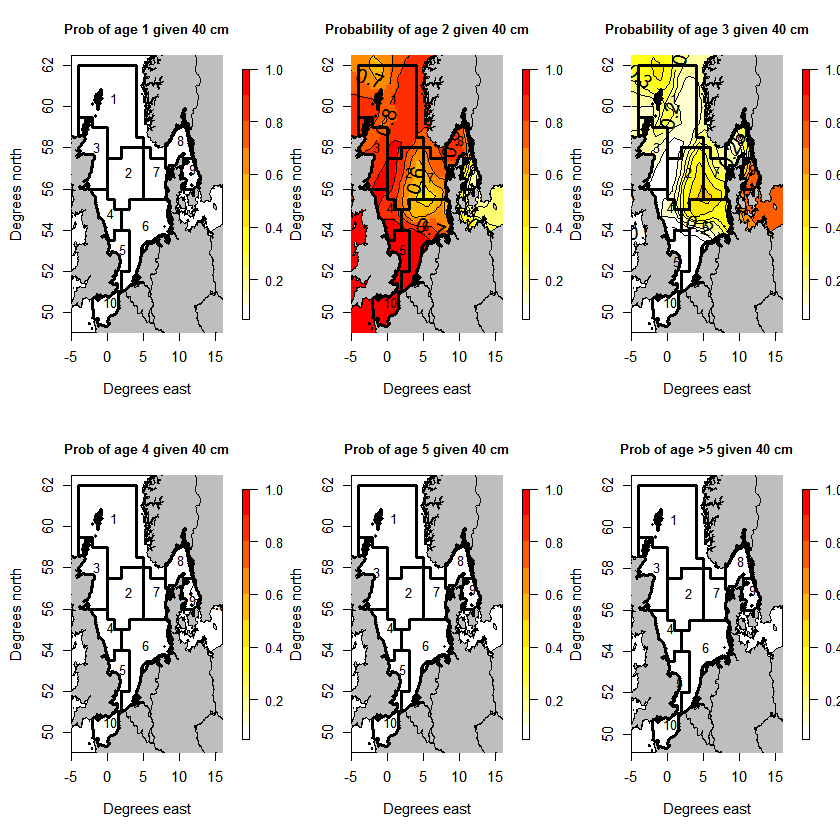
\includegraphics[scale=0.4]{Allcode40cm2015.png}
%\caption{Estimated probability of age of a 40 cm long cod in the first quarter of year 2015. The probability of age three or older is approximately zero. The polygones marked 1 to 10 is the round fish areas (RFAs) where the ALK is assumed constant in the currently used estimators of the official CPUEs.}\label{fig:40cmCod2015}
%\end{figure}

%\begin{figure}[h!]
%  \centering
% {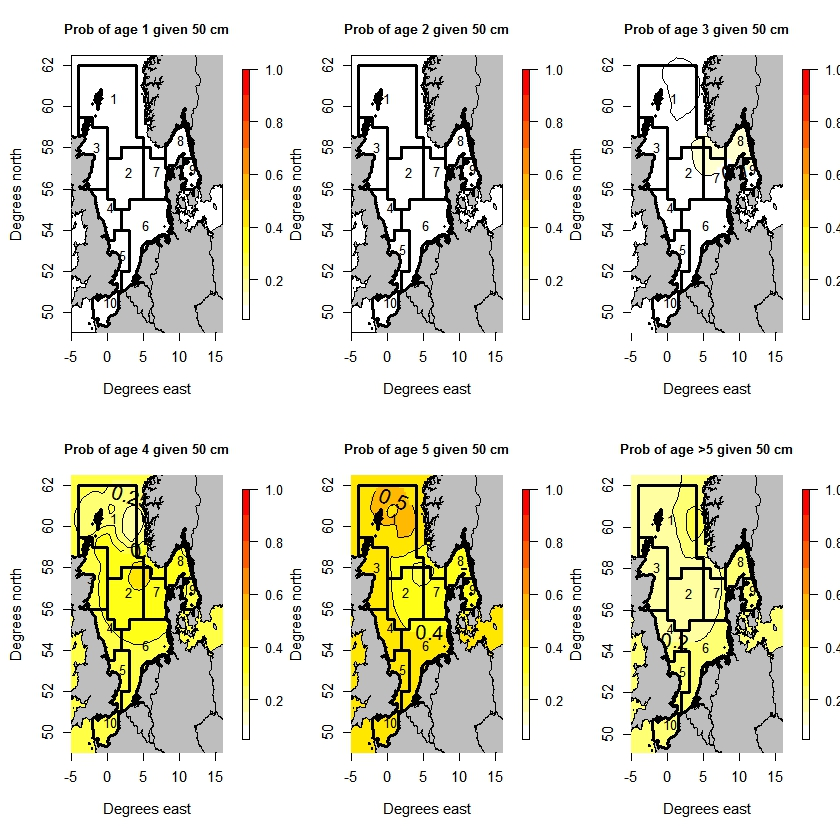
\includegraphics[scale=0.4]{saithe2015Q1Map.jpeg}}   
% \captionsetup{font= footnotesize, width=15cm}{
% \caption{Estimated probability of age of a 50 cm long saithe in the first quarter of year 2015. The probability of age 1 to age 3 is approximately zero. The polygones marked 1 to 10 is the round fish areas (RFAs) where the ALK is assumed constant in the currently used estimators of the official CPUEs. The plots show that the age of saithe is more likely to be 5 given that it is 50 cm, particularly in RFA 1.}\label{saithe2015Q1Map}}
%\end{figure}


%\clearpage
%
%
%Otoliths are usually collected from a fraction of the fish sampled (see Table \ref{tab:otolithsTable} in appendix \ref{secAp:otolithappendix}), but in some cases only a small number of fish are caught so otoliths are taken from all catches. ({\bf include legend on plots and number of trawl hauls with length only and age data})
%
%\begin{figure}[h!]
%    \centering
%\subfloat{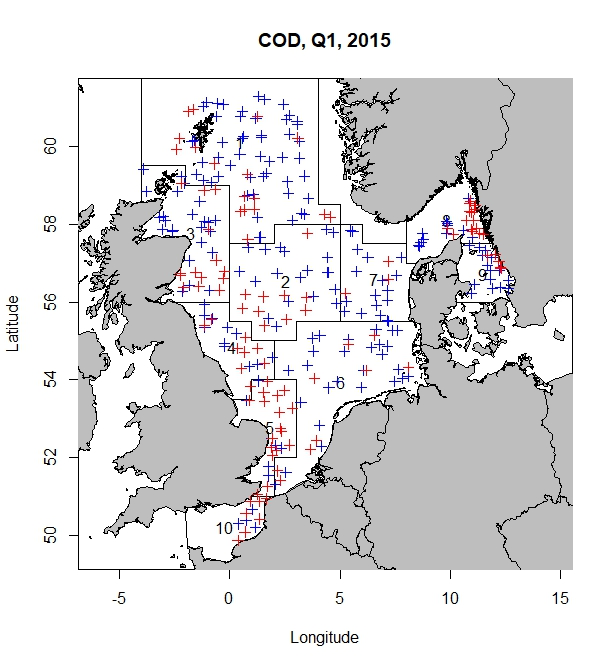
\includegraphics[width=.43\linewidth]{codQ12015Hauls.jpeg}}
%    \hfill
%\subfloat{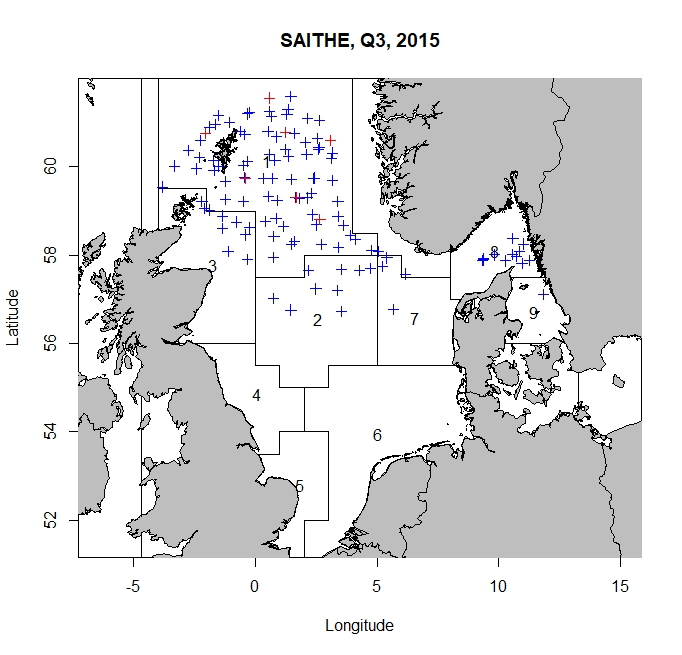
\includegraphics[width=.48\linewidth]{saitheQ32015Hauls.jpeg}}
%
%\subfloat{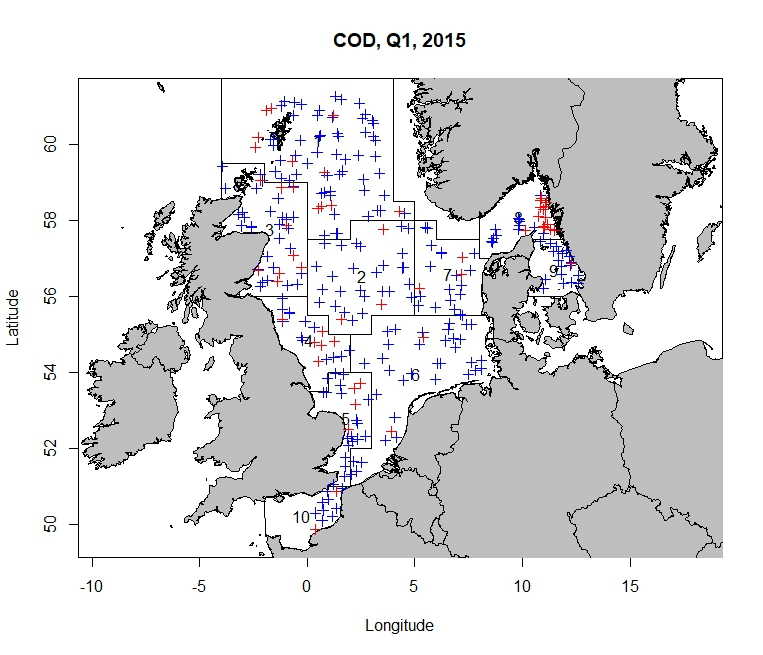
\includegraphics[width=.48\linewidth]{codQ12015Hauls5cm.jpeg}}
%    \hfill
%\subfloat{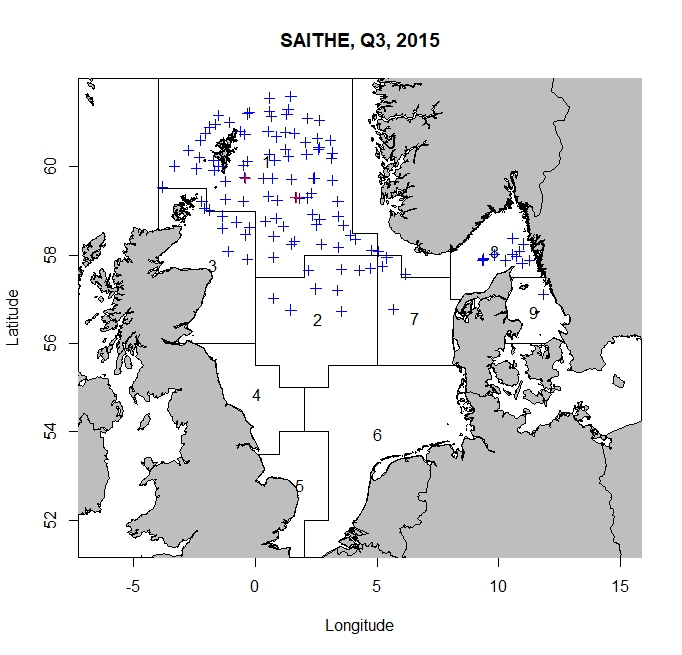
\includegraphics[width=.44\linewidth]{saitheQ32015Hauls5cm.jpeg}}\
%    \caption{cod with length class 1 cm (upper left) and length class 5 cm (lower left), and saithe with length class 1cm (upper right) and length class 5 cm (lower right)}
%    \label{fig:trawlhauls}
%\end{figure}
%
%
%\clearpage
%\section{RESULTS}
%\label{sec:results}
%
%In this section we show differences between the estimated CPUE with the proposed procedures. We further show how much information which would typically have been lost if the number of otholits investigated were reduced as explained in section \ref{sec:optimizationsampling}.
%
%Before we show the estimated CPUE we want to highlight some results from the model based ALK. 
%
%\subsection{Estimates of abundance-at-age and their uncertainty}
%\label{sec:resultsabundance}
%%The model-based ALK estimator gives the best overall estimation of uncertainty of estimated CPUE as it accounts for spatial differences in age-length structure. As expected the DATRAS estimator gives smaller estimates of the uncertainty in all ages, except ages 3 and 4. The DATRAS ALK estimator lacks the potential to account for spatial differences in the age-length structure, which may be as a consequence of differential growth rates or size-specific migration. The haul-based ALK estimator gives comparable estimates with the the model-based ALK estimator but uncertainty estimates are generally smaller. For all four bootstrap approaches estimated CPUE for all ages is captured within a $95\%$ confidence interval. Note that the nonparametric bootstrap method is advantageous  because it does not assume any distribution for the data, and it also accounts for some of the variability in the sampling distribution of the CPUE, however, there are some limitations of this method. The most important limitation is the assumption that the distribution of the data represented by the sample is a reasonable estimate of the population function from which the data are sampled. If this assumption is violated the random sampling  performed in the bootstrap procedure may add another level of sampling error, resulting in invalid statistical estimations \citep{haukoos2005advanced}. As discussed in Section \ref{overview} the selection of the trawling locations in IBTS is semi-random where cruise leaders selects "clear" tow locations or "blind" tow locations if no clear tow exists by checking the proposed trawl track for hazardous seabed obstructions with acoustic methods. More recently selection of tow locations is based on pre-proposed valid tow locations with start and end positions executed in the period 2000-2017. Hence, the lack of a fully randomized sampling process has the potential to result in biased estimates of parameters and their uncertainty. Random sampling performed in the bootstrap procedure also adds another level of potential sampling error, which is reflected in variation and biased estimates commonly performed in the bootstrap analysis. Note that the sampling distribution of the bootstrapped statistics is frequently not symmetric and computing point estimates from in this manner may reflect biased estimation from the samples. This can be seen in the estimated bootstrap mean values in Table \ref{resultstable}. The percentile method adopted for computing confidence intervals implicitly assumes the sampling distribution of the bootstrapped statistic is symmetric, and a violation of this assumption would caused the coverage to be substantial %(\emph{possibly include median estimates of CPUE to check for skewness or symmetry, and make reference to it. The percentile method also does partial skewness correction, which adds random variability. Possibly check for significant difference between estimates from different estimators? Approximate confidence intervals - as exact nonparametric confidence intervals do not exist for most parameters \citep{bahadur1956nonexistence}}). 
%
%
%
%
%\begin{tiny}
%\begin{table}[h!]
%\centering
%\scriptsize
%\setlength\tabcolsep{1.8pt} 
%\captionsetup{font=small, width = 16.5cm}{
%\caption{Estimates of abundance indices (Index), and estimated standard errors for 400 bootstrap samples from the following bootstrap procedures: DATRAS, Naive, Stratified, and Hierarchical for cod in RFA 1 in the first quarter of year 2015. Approximate $95 \%$ confidence intervals (CI) are also given.}\label{resultstablesaithe}}
%\begin{tabular}{ccccccccccccccccccccccccccc}
%\hline \\[0.1ex]
%  & \multicolumn{3}{c}{\bf DATRAS ALK} & \multicolumn{3}{c}{\thead{\bf Haul-based ALK }} & \multicolumn{3}{c}{\thead{\bf  Model-based ALK}} \\[1.5ex]
%  & \multicolumn{3}{c}{DATRAS Bootstrap}   & \multicolumn{3}{c}{Stratified Bootstrap}   & \multicolumn{3}{c}{Stratified Bootstrap} \\[1.5ex]
%   \cmidrule(lr{0.5em}){2-4}  \cmidrule(lr{0.1em}){5-7} \cmidrule(lr{0.5em}){8-10}  \\ [0.1ex]
%{\bf Age ($a$) }  &\thead{Abundance \\ estimate} & \thead{Standard \\ error} & \thead{Relative \\ standard error} &\thead{Abundance \\ estimate} & \thead{Standard \\ error} & \thead{Relative \\ standard error} & \thead{Abundance \\ Estimate}  & \thead{Standard \\ error} & \thead{Relative \\ standard error}& \\[0.5ex]
%\cmidrule(lr{0.5em}){1-1}  \cmidrule(lr{0.5em}){2-4}  \cmidrule(lr{0.1em}){5-7} \cmidrule(lr{0.5em}){8-10}  \\ [0.1ex]
%0  & 0      & 0    & $-$  & 0    &   0   & $-$     & 0    & 0    & $-$         \\[1ex]
%1  & 0.764  & 0.26 & $34 \%$ & 0.60  & 0.24 & $40 \%$   & 0.70  & 0.36 & $51 \%$   \\[1ex]
%2  & 21.989 & 6.76 & $31 \%$ & 22.21 & 4.15 & $19 \%$   & 22.11 & 4.28 & $19 \%$   \\[1ex]
%3  & 11.285 & 2.19 & $19 \%$ & 10.58 & 1.20 & $11 \%$   & 10.99 & 1.77 & $16 \%$ \\[1ex]
%4  & 3.265  & 0.71 & $22 \%$ & 3.67  & 1.28 & $35 \%$   & 3.50  & 0.87 & $25 \%$  \\[1ex]
%5  & 1.147  & 0.34 & $30 \%$ & 1.27  & 0.42 & $33 \%$   & 1.20  & 0.48 & $40 \%$  \\[1ex]
%6+  & 1.276  & 0.38 & $30 \%$ & 1.40  & 0.70 & $50 \%$   & 1.21  & 0.42 & $35 \%$  \\[4.5ex]
%
%
% & \multicolumn{8}{c}{\bf Approximate $95 \%$ CI from bootstrap procedures} \\[1.5ex]
%0  & 0      &(0, 0)         && 0      &  (0, 0)         && 0     & (0, 0)           \\[1ex]
%1  & 0.764  &(0.31, 1.33)   && 0.60   &  (0.31, 0.91)   && 0.70  & (0.35, 1.48)    \\[1ex]
%2  & 21.898 &(12.73, 37.15) && 22.21  &  (15.64, 30.72) && 22.11 & (14.76, 30.36) \\[1ex]
%3  & 11.285 &(6.31, 15.02)  && 10.58  &  (8.74, 13.65)  && 10.99 & (8.61, 15.42)  \\[1ex]
%4  & 3.265  &(1.49, 4.21)   && 3.67   &  (2.81, 4.74)   && 3.50  &(1.96, 5.60)   \\[1ex]
%5  & 1.147  &(0.40, 1.75)   && 1.27   &  (0.67, 2.31)   && 1.20  &  (0.56, 2.78)   \\[1ex]
%6+  & 1.276  &(0.44, 1.82)   && 1.40   &  (0.78, 2.69)   && 1.21  & (0.70, 2.43)  \\[1ex]
%\hline
%\end{tabular}
%\end{table}
%\end{tiny}
%
%
%
%
%
%\begin{tiny}
%\begin{table}[h!]
%\centering
%\scriptsize
%\setlength\tabcolsep{1.8pt} 
%\captionsetup{font=small, width = 16.5cm}{
%\caption{Estimates of abundance indices (Index), and estimated standard errors for 400 bootstrap samples from the following bootstrap procedures: DATRAS, Naive, Stratified, and Hierarchical for cod in RFA 1 in the first quarter of year 2015. Approximate $95 \%$ confidence intervals (CI) are also given.}\label{resultstablesaithe}}
%\begin{tabular}{ccccccccccccccccccccccccccc}
%\hline \\[0.1ex]
%  & \multicolumn{3}{c}{\bf DATRAS ALK} & \multicolumn{4}{c}{\thead{\bf Haul-based ALK }} & \multicolumn{4}{c}{\thead{\bf  Model-based ALK}} \\[1.5ex]
%{\bf Age ($a$) }  &Index & DATRAS &  Naive &Index & Naive & Stratified &  Hierarchical &Index & Naive &Stratified &  Hierarchical & \\[0.5ex]
%\cmidrule(lr{0.5em}){1-1}  \cmidrule(lr{0.5em}){2-4}  \cmidrule(lr{0.1em}){5-8} \cmidrule(lr{0.5em}){9-12}  \\ [0.1ex]
%1  & 0      & 0    & 0            & 0    &   0  & 0     & 0     & 0           & 0         &  0   & 0       \\[1ex]
%2  & 0.764  & 0.26 & 0.23 & 0.60  & 0.24 & 0.16 & 0.81  & 0.70  & 0.36 & 0.31 & 0.78   \\[1ex]
%3  & 21.989 & 6.76 & 4.08 & 22.21 & 4.15 & 4.20 & 13.23 & 22.11 & 4.28 & 4.26 & 10.69  \\[1ex]
%4  & 11.285 & 2.19 & 1.27 & 10.58 & 1.20 & 1.28 & 5.85  & 10.99 & 1.77 & 1.84 & 4.53 \\[1ex]
%5  & 3.265  & 0.71 & 0.57 & 3.67  & 1.28 & 0.56 & 3.02  & 3.50  & 0.87 & 0.94 & 2.46 \\[1ex]
%6  & 1.147  & 0.34 & 0.33 & 1.27  & 0.43 & 0.43 & 1.59  & 1.20  & 0.48 & 0.62 & 0.83 \\[1ex]
%7  & 1.276  & 0.38 & 0.39 & 1.40  & 0.70 & 0.53 & 2.01  & 1.21  & 0.42 & 0.46 & 0.85 \\[4.5ex]
%
%
% &&& \multicolumn{8}{c}{\bf Approximate $95 \%$ CI from bootstrap procedures} \\[1.5ex]
%1  & 0      &(0, 0)         & (0, 0)        & 0     &(0, 0)         &  (0, 0)         & (0, 0)        & 0     &(0, 0)        & (0, 0)         & (0, 0)   \\[1ex]
%2  & 0.764  &(0.31, 1.33)   & (0.40, 1.22)  & 0.60  &(0.20, 1.18)   &  (0.31, 0.91)   & (0, 3.81)     & 0.70  &(0.37, 1.81)  & (0.35, 1.48)   & (0.05, 2.05) \\[1ex]
%3  & 21.898 &(12.73, 37.15) & (14.90, 30.01)& 22.21 &(15.01, 30.09) &  (15.64, 30.72) & (11.34, 61.57)& 22.11 &(14.56, 30.61)& (14.76, 30.36) & (7.12, 41.41)\\[1ex]
%4  & 11.285 &(6.31, 15.02)  & (9.63, 14.42) & 10.58 &(8.75, 13.54)  &  (8.74, 13.65)  & (0, 17.73)    & 10.99 &(8.45, 15.43) & (8.61, 15.42)  & (3.90, 19.99)\\[1ex]
%5  & 3.265  &(1.49, 4.21)   & (2.45, 4.50)  & 3.67  &(2.42, 7.35)   &  (2.81, 4.74)   & (0, 8.26)     & 3.50  &(2.11, 5.56)  & (1.96, 5.60)   & (0.87, 8.10)\\[1ex]
%6  & 1.147  &(0.40, 1.75)   & (0.67, 1.95)  & 1.27  &(0.50, 2.14)   &  (0.67, 2.31)   & (0, 4.35)     & 1.20  & (0.58, 2.50) & (0.56, 2.78)   & (0.15, 2.98)\\[1ex]
%7  & 1.276  &(0.44, 1.82)   & (0.72, 2.24)  & 1.40  &(0.71, 3.42)   &  (0.78, 2.69)   & (0, 5.15)     & 1.21  &(0.70, 2.27)  & (0.70, 2.43)   & (0.09, 3.22) \\[1ex]
%\hline
%\end{tabular}
%\end{table}
%\end{tiny}
%
%\clearpage
%
%%\clearpage
%\begin{small}
%\begin{table}[h!]
%\centering
%\scriptsize
%\setlength\tabcolsep{1.8pt} 
%\captionsetup{font=small, width = 16.5cm}{
%\caption{Estimates of abundance indices (Index), and estimated standard errors for 200 bootstrap samples from the following bootstrap procedures: DATRAS, Naive, Stratified, and Hierarchical for cod in RFA 1 in the first quarter of year 2015. Approximate $95 \%$ confidence intervals (CI) are also given.}\label{resultstablesaithe}}
%\begin{tabular}{ccccccccccccccccccccccccccc}
%\hline \\[0.1ex]
%  & \multicolumn{3}{c}{\bf DATRAS ALK} & \multicolumn{4}{c}{\thead{\bf Haul-based ALK }} & \multicolumn{4}{c}{\thead{\bf  Model-based ALK}} \\[1.5ex]
%{\bf Age ($a$) }  &Index & DATRAS &  Naive &Index & Naive & Stratified &  Hierarchical &Index & Naive &Stratified &  Hierarchical & \\[0.5ex]
%\cmidrule(lr{0.5em}){1-1}  \cmidrule(lr{0.5em}){2-4}  \cmidrule(lr{0.1em}){5-8} \cmidrule(lr{0.5em}){9-12}  \\ [0.1ex]
%1  & 0     & 0         & 0          & 0    &   0  & 0         & 0         & 0         & 0         &  0   & 0       \\[1ex]
%2  & 0.764  & 0.26 & 0.24 & 0.60  & 0.23 & 0.17 & 2.55 & 0.70  & 0.34 & 0.45 & 0.48   \\[1ex]
%3  & 21.989 & 7.30 & 3.89 & 22.21 & 4.14 & 4.19 & 9.61 & 22.11 & 4.46 & 4.10 & 13.23  \\[1ex]
%4  & 11.285 & 2.29 & 1.30 & 10.58 & 1.18 & 1.29 & 4.72 & 10.99 & 2.37 & 1.94 & 5.20 \\[1ex]
%5  & 3.265  & 0.74 & 0.57 & 3.67  & 1.18 & 0.58 & 2.00 & 3.50  & 0.93 & 0.89 & 3.28 \\[1ex]
%6  & 1.147  & 0.35 & 0.37 & 1.27  & 0.42 & 0.42 & 0.91 & 1.20  & 0.46 & 0.56 & 1.28 \\[1ex]
%7  & 1.276  & 0.41 & 0.40 & 1.40  & 0.73 & 0.52 & 0.85 & 1.21  & 0.42 & 0.43 & 2.63 \\[4.5ex]
%
%
% &&& \multicolumn{8}{c}{\bf Approximate $95 \%$ CI from bootstrap procedures} \\[1.5ex]
%1  & 0      &(0, 0)          & (0, 0)        & 0     &(0, 0)          &  (0, 0)          & (0, 0)       & 0     &(0, 0) & (0, 0)         & (0, 0)          & \\[1ex]
%2  & 0.764  & (0.27, 1.29)   & (0.40, 1.34)  & 0.60  &(0.31, 1.15)    &  (0.31, 0.93)    & (0, 7.22)    & 0.70  &(0.40, 1.72)  & (0.38, 1.89)   & (0.02, 1.72) \\[1ex]
%3  & 21.898 & (12.70, 37.67) & (15.46, 29.63)& 22.21 & (15.22, 30.25) &  (14.65, 30.18)  & (3.65, 40.02)& 22.11 &(14.33, 3097) & (14.71, 29.90) & (3.71, 54.91)\\[1ex]
%4  & 11.285 &(6.64, 15.33)   & (9.47, 14.32) & 10.58 &(8.94, 13.54)   &  (9.14, 13.94)   & (0, 15.63)   & 10.99 &(8.44, 16.60) & (8.65, 16.07)  & (1.84, 21.53)\\[1ex]
%5  & 3.265  &(1.56, 4.46)    & (2.43, 4.39)  & 3.67  &(2.46, 6.59)    &  (2.75, 4.77)    & (0, 7.18)    & 3.50  &(2.18, 5.30)  & (1.92, 5.07)   & (0.10, 10.07)\\[1ex]
%6  & 1.147  &(0.39, 1.77)    & (0.64, 1.96)  & 1.27  & (0.39, 2.02)   &  (0.69, 2.27)    & (0, 3.83)    & 1.20  & (0.54, 2.39)  & (0.60, 2.79)   & (0.01, 3.30)\\[1ex]
%7  & 1.276  &(0.42, 2.13)    & (0.75, 2.28)  & 1.40  &(0.62, 3.23)    &  (0.78, 2.68)    & (0, 2.38)    & 1.21  &(0.70, 2.30)  & (0.66, 2.26)   & (0., 3.09) \\[1ex]
%\hline
%\end{tabular}
%\end{table}
%\end{small}
%
%
%
%%\clearpage
%\begin{small}
%\begin{table}[h!]
%\centering
%\scriptsize
%\setlength\tabcolsep{1.8pt} 
%\captionsetup{font=small, width = 16.5cm}{
%\caption{Estimates of abundance indices (Index), and estimated standard errors from the following bootstrap procedures: DATRAS, Naive, Stratified, and Hierarchical for saithe in RFA 1 in the third quarter of year 2015. Approximate $95 \%$ confidence intervals (CI) are also given.}\label{resultstablesaithe}}
%\begin{tabular}{ccccccccccccccccccccccccccc}
%\hline \\[0.1ex]
%  & \multicolumn{3}{c}{\bf DATRAS ALK} & \multicolumn{4}{c}{\thead{\bf Haul-based ALK }} & \multicolumn{4}{c}{\thead{\bf  Model-based ALK}} \\[1.5ex]
%{\bf Age ($a$) }  &Index & DATRAS &  Naive &Index & Naive & Stratified &  Hierarchical &Index & Naive &Stratified &  Hierarchical & \\[0.5ex]
%\cmidrule(lr{0.5em}){1-1}  \cmidrule(lr{0.5em}){2-4}  \cmidrule(lr{0.1em}){5-8} \cmidrule(lr{0.5em}){9-12}  \\ [0.1ex]
%1  & 0     & 0         & 0          & 0    &   0  & 0         & 0         & 0         & 0         &  0   & 0       \\[1ex]
%2  & 0.764  & 0.26 & 0.24 & 0.60  & 0.23 & 0.17 & 2.55 & 0.70  & 0.34 & 0.45 & 0.48   \\[1ex]
%3  & 21.989 & 7.30 & 3.89 & 22.21 & 4.14 & 4.19 & 9.61 & 22.11 & 4.46 & 4.10 & 13.23  \\[1ex]
%4  & 11.285 & 2.29 & 1.30 & 10.58 & 1.18 & 1.29 & 4.72 & 10.99 & 2.37 & 1.94 & 5.20 \\[1ex]
%5  & 3.265  & 0.74 & 0.57 & 3.67  & 1.18 & 0.58 & 2.00 & 3.50  & 0.93 & 0.89 & 3.28 \\[1ex]
%6  & 1.147  & 0.35 & 0.37 & 1.27  & 0.42 & 0.42 & 0.91 & 1.20  & 0.46 & 0.56 & 1.28 \\[1ex]
%7  & 1.276  & 0.41 & 0.40 & 1.40  & 0.73 & 0.52 & 0.85 & 1.21  & 0.42 & 0.43 & 2.63 \\[4.5ex]
%
%
% &&& \multicolumn{8}{c}{\bf Approximate $95 \%$ CI from bootstrap procedures} \\[1.5ex]
%1  & 0      &(0, 0)          & (0, 0)        & 0     &(0, 0)          &  (0, 0)          & (0, 0)       & 0     &(0, 0) & (0, 0)         & (0, 0)          & \\[1ex]
%2  & 0.764  & (0.27, 1.29)   & (0.40, 1.34)  & 0.60  &(0.31, 1.15)    &  (0.31, 0.93)    & (0, 7.22)    & 0.70  &(0.40, 1.72)  & (0.38, 1.89)   & (0.02, 1.72) \\[1ex]
%3  & 21.898 & (12.70, 37.67) & (15.46, 29.63)& 22.21 & (15.22, 30.25) &  (14.65, 30.18)  & (3.65, 40.02)& 22.11 &(14.33, 3097) & (14.71, 29.90) & (3.71, 54.91)\\[1ex]
%4  & 11.285 &(6.64, 15.33)   & (9.47, 14.32) & 10.58 &(8.94, 13.54)   &  (9.14, 13.94)   & (0, 15.63)   & 10.99 &(8.44, 16.60) & (8.65, 16.07)  & (1.84, 21.53)\\[1ex]
%5  & 3.265  &(1.56, 4.46)    & (2.43, 4.39)  & 3.67  &(2.46, 6.59)    &  (2.75, 4.77)    & (0, 7.18)    & 3.50  &(2.18, 5.30)  & (1.92, 5.07)   & (0.10, 10.07)\\[1ex]
%6  & 1.147  &(0.39, 1.77)    & (0.64, 1.96)  & 1.27  & (0.39, 2.02)   &  (0.69, 2.27)    & (0, 3.83)    & 1.20  & (0.54, 2.39)  & (0.60, 2.79)   & (0.01, 3.30)\\[1ex]
%7  & 1.276  &(0.42, 2.13)    & (0.75, 2.28)  & 1.40  &(0.62, 3.23)    &  (0.78, 2.68)    & (0, 2.38)    & 1.21  &(0.70, 2.30)  & (0.66, 2.26)   & (0., 3.09) \\[1ex]
%\hline
%\end{tabular}
%\end{table}
%\end{small}
%
%
%\subsection{Optimum Sampling Effort for North Sea cod and saithe}
%\label{sec:resultsoptim}
%


\clearpage

\section{DISCUSSION}
\label{sec:discussion}
\begin{itemize}
\item We have investigated three ALK estimators: 1) DATRAS ALK, 2)Haul-based ALK and 3) Model-based ALK
\item discuss ALK estimators, which of the three is the most appropriate at this time, discuss  model-based ALK and compare with \citet{berg2012spatial} as they are similar are both used on IBTS data
\item How can estimators be improved, also computational time (1000 bootstrapped samples for each of the four estimators took hours (possibly more than ten, needs verification))
\item Possibly consider hierarchical bootstrapping as done in \citet{ren2010nonparametric} - draft codes are available
\item Discuss next steps for example, removal of otoliths or age information and trawl hauls: the effect may be substantial for larger fish (hence older fish) - as shown in table \ref{agelengthcomposition} fewer older fish are sampled and many younger ones are sampled so the effect would be marginal for younger fish). Draft codes are available for this. \citet{wieland2009estimating} found that considerable catches for cod of older ages were made where the IBTS reported low densities or no cod all (\emph{this is based on data from collaborative fishermen-biologists project on cod in the north-eastern central North Sea}). Also smaller sample sizes would also have an effect on estimated bootstrapped confidence intervals. The smaller the original sample the less likely it is to represent the entire population, thus the more difficult it becomes to compute valid confidence intervals. The bootstrap relies heavily on the tails of the estimated sampling distribution when computing confidence intervals, and using small samples may jeopardize the validity of this computation.  
\item a possible full model-based approach for estimating abundance at age with variance simultaneously?
\item \emph{Note to us: include ICES references}
\end{itemize}



\clearpage

\bibliographystyle{apalike}
\bibliography{ibtsBib}

\clearpage

\appendix


\clearpage
\section{\large Areas fished by different countries in the North Sea IBTS}
\label{secAp:areasfishedappendix}
Typically, two different countries fish each rectangle so that at least two trawl hauls are made per rectangle. But, intensified sampling is carried out in the following areas: at least 3 hauls per rectangle are taken in statistical rectangles  31F1, 31F2, 32F1, 33F4, 34F2, 34F3, 34F4, 35F3, 35F4; while six or more hauls per rectangle are taken in statistical rectangles  30F1, 32F2, 32F3, 33F2, 33F3 (ICES 1999).  The Skagerrak and Kattegat is fished solely by Sweden, who sample more than once in every rectangle while the west of Shetland (in Q1 and Q3) and inshore areas (Q3) is fished solely by Scotland. The edge of the Norwegian Trench is fished solely by Norway, but inshore areas near Denmark is fished by Denmark. The southern North Sea is fished by Denmark, Germany and England. France, typically, is the only country that surveys the western English Channel. Areas are surveyed by a single country because of the large proportion of untrawalable area (and subsequent gear damage issues experienced by other nations)  for efficient logistical purposes. Table \ref{countries} gives the countries and research vessels participating the North Sea IBTS.\\
\begin{small}
\begin{table}[h!]
\centering
\captionsetup{font=small, width = 15.5cm}{
\caption{Survey countries, vessel name, and period research vessels participating in first quarter (Q1) and third quarter (Q3) during 1997-2017.}\label{countries}}
\begin{tabular}{cccccccc}
\hline \\[0.1ex]
  & \multicolumn{2}{c}{\bf First Quarter (Q1)} & \multicolumn{2}{c}{\bf Third Quarter (Q3)}\\[1.5ex]
{\bf Country }  & Vessel name & Period    & Vessel name & Period  \\[0.5ex]
\hline \\[0.5ex]
Denmark  &   Dana   &   January-February  & Dana & July-August    \\[1ex]
France  & Thalassa II & January-February & - & -   \\[1ex]
Germany   &  Walther  Herwig III & January-February   &   Walther  Herwig III & July-August \\[1ex]
Netherlands &  Tridens 2 &  January-February   & - & -     \\[1ex]
Norway  &   G.O. Sars  & January-February &    Johan Hjort  & July   \\[1ex]
UK England &- & -&  Endeavour &  August-September  \\[1ex]
UK Scotland   &  Scotia III &  January-February & Scotia III &  July-August \\[1ex]
Sweden  &  Dana &  January-February  &  Dana &  August                  \\[0.5ex]
\hline
\end{tabular}
\end{table}
\end{small}

\section{\large Otolith sampling per fish species}
\label{secAp:otolithappendix}
From 1991-2017, most countries conducted quota sampling of otoliths per length group in a RFA. But from 2013 Norway has been sampling one otolith per length class from each trawl haul (to 0.1$\cm$ below for shellfish, to 0.5$\cm$ below for herring and sprat and to 1$\cm$ below for all other species). From the first quarter in 2018 all countries are required to sample one otolith per length class per trawl haul.  Table \ref{tab:otolithsTable} gives the minimum sampling levels of otoliths for the target species. However, for the smallest size groups, that presumably contain only one age group, the number of otoliths per length class may be reduced, and more otoliths per length are required for the larger length classes. \\
%\clearpage
\begin{small}
\begin{table}[h!]
\centering
\caption{Minimum sampling levels of otoliths by species for RFA or per trawl haul.}
\label{tab:otolithsTable}
\begin{tabularx}{\linewidth}{r l l l l X}
\toprule 
Period &  Species  & Minimum sampling levels of otoliths per length class    \\[0.7ex]
\midrule \\[0.1ex]
{\bf 1991-2017} & & {\bf Number of otoliths per length class in a RFA}  \\[1.8ex]
     & herring  &  $8$  otoliths per $\frac{1}{2}$ cm group \\[0.8ex]
     & sprat    & $16$  otoliths per $\frac{1}{2}$ cm length class  $8.0 -11.0$ cm\\[0.8ex]
              & & $12$  otoliths per $\frac{1}{2}$ cm length class  $\geq 11.0$ cm\\[0.8ex]
& mackerel      & $8$  otoliths per $\frac{1}{2}$ cm length class \\[0.8ex]
& cod       	  & $8$  otoliths per $1$ cm length class\\[0.8ex]
&haddock   	  & $8$  otoliths per $1$ cm length class \\[0.8ex]
&whiting    	  & $8$  otoliths per $1$ cm length class \\[0.8ex]
&Norway pout   & $8$  otoliths per $1$ cm length class\\[0.8ex]
&saithe        & $8$  otoliths per $1$ cm length class \\[2ex] 
& All target species      &  From 2013 Norway and Scotland, and  Netherlands from 2016 \\[0.7ex] 
&& have been sampling 1 otolith per length class from each trawl haul \\[0.7ex] 
&& (to 0.1$\cm$ below for shellfish, to 0.5$\cm$ below for herring and sprat, and \\ [0.7ex] 
&& to 1$\cm$ below for all other species).\\[2.7ex] 

{\bf 2018} & & {\bf Number of otoliths per length class per trawl haul}  \\[1.8ex]
  & herring  &  $1$  otolith per $\frac{1}{2}$ cm group \\[0.8ex]
     & sprat    & $1$  otolith per $\frac{1}{2}$ cm length class  $8.0 -11.0$ cm\\[0.8ex]
              & & $1$  otolith per $\frac{1}{2}$ cm length class  $\geq 11.0$ cm\\[0.8ex]
& mackerel      & $1$  otolith per $1$ cm length class \\[0.8ex]
& cod       	  & $1$  otolith per $1$ cm length class\\[0.8ex]
& haddock & $2$  otoliths per $5$ cm length class $11 -15, \ 16-20, \ 21-25, \ 26-30$ cm \\[0.8ex]
& Norway pout & $2$  otoliths per $5$ cm length class $5 -10, \ 11-15$ cm\\[0.8ex]
               & & $2$  otoliths per $1$ cm length class $> 15$ cm\\[1.8ex]
&saithe        & $1$  otolith per $1$ cm length class \\[0.8ex]  
&plaice       & $1$  otolith per $1$ cm length class \\[0.5ex]
\bottomrule         
\end{tabularx}
\end{table}
\end{small}

%\clearpage
 \section{\large Weightings of Statistical Rectangles}
 \label{secAp:weightings}
%\clearpage 
 \begin{small}
\begin{table}[h!]
\centering
\caption{Weights used for Pollachius virens in equation (\ref{eq:cpueRec}).}
\begin{footnotesize}
\begin{tabular}{clclclclcl}
  \hline \\ [0.3ex]
 StatRec & Weight & StatRec & Weight & StatRec & Weight & StatRec & Weight & StatRec & Weight  \\ [1.0ex]
  \hline \\ [0.3ex]
 31F1 &  0.6 & 38F0 &    1 & 41F7 &    1 & 44F3 &    1 & 48E7 &    1 \\ 
 31F2 &  0.8 & 38F1 &    1 & 41F8 &  0.1 & 44F4 &    1 & 48E8 &  0.9 \\ 
 31F3 & 0.05 & 38F2 &    1 & 41G0 &  0.2 & 44F5 &  0.9 & 48E9 &    1 \\ 
 32F1 &  0.8 & 38F3 &    1 & 41G1 & 0.97 & 44F8 & 0.25 & 48F0 &    1 \\ 
 32F2 &    1 & 38F4 &    1 & 41G2 & 0.53 & 44F9 &  0.8 & 48F1 &    1 \\ 
 32F3 &  0.8 & 38F5 &    1 & 42E7 &  0.4 & 44G0 & 0.94 & 48F2 &    1 \\ 
 32F4 & 0.01 & 38F6 &    1 & 42E8 &    1 & 44G1 &  0.6 & 48F3 &  0.5 \\ 
 33F1 &  0.3 & 38F7 &    1 & 42E9 &    1 & 45E6 &  0.4 & 48G0 & 0.02 \\ 
 33F2 &    1 & 38F8 &  0.3 & 42F0 &    1 & 45E7 &    1 & 49E6 &  0.8 \\ 
 33F3 &    1 & 39E8 &  0.5 & 42F1 &    1 & 45E8 &    1 & 49E7 &    1 \\ 
 33F4 &  0.4 & 39E9 &    1 & 42F2 &    1 & 45E9 &    1 & 49E8 &  0.4 \\ 
 34F1 &  0.4 & 39F0 &    1 & 42F3 &    1 & 45F0 &    1 & 49E9 &    1 \\ 
 34F2 &    1 & 39F1 &    1 & 42F4 &    1 & 45F1 &    1 & 49F0 &    1 \\ 
 34F3 &    1 & 39F2 &    1 & 42F5 &    1 & 45F2 &    1 & 49F1 &    1 \\ 
 34F4 &  0.6 & 39F3 &    1 & 42F6 &    1 & 45F3 &    1 & 49F2 &    1 \\ 
 35F0 &  0.8 & 39F4 &    1 & 42F7 &    1 & 45F4 &  0.6 & 49F3 &  0.5 \\ 
 35F1 &    1 & 39F5 &    1 & 42F8 &  0.2 & 45F8 &  0.3 & 50E6 &  0.1 \\ 
 35F2 &    1 & 39F6 &    1 & 42G0 & 0.32 & 45F9 & 0.02 & 50E7 &  0.6 \\ 
 35F3 &    1 & 39F7 &    1 & 42G1 & 0.89 & 45G0 & 0.24 & 50E8 &  0.7 \\ 
 35F4 &  0.9 & 39F8 &  0.4 & 42G2 & 0.64 & 45G1 & 0.55 & 50E9 &  0.9 \\ 
 35F5 &  0.1 & 40E7 & 0.04 & 43E7 & 0.03 & 46E6 &  0.4 & 50F0 &    1 \\ 
 36F0 &  0.9 & 40E8 &  0.8 & 43E8 &  0.9 & 46E7 &  0.9 & 50F1 &    1 \\ 
 36F1 &    1 & 40E9 &    1 & 43E9 &    1 & 46E8 &    1 & 50F2 &    1 \\ 
 36F2 &    1 & 40F0 &    1 & 43F0 &    1 & 46E9 &    1 & 50F3 &  0.2 \\ 
 36F3 &    1 & 40F1 &    1 & 43F1 &    1 & 46F0 &    1 & 51E6 &    0 \\ 
 36F4 &    1 & 40F2 &    1 & 43F2 &    1 & 46F1 &    1 & 51E7 &    0 \\ 
 36F5 &    1 & 40F3 &    1 & 43F3 &    1 & 46F2 &    1 & 51E8 &  0.5 \\ 
 36F6 &  0.9 & 40F4 &    1 & 43F4 &    1 & 46F3 &  0.8 & 51E9 &    1 \\ 
 36F7 &  0.4 & 40F5 &    1 & 43F5 &    1 & 46F9 &  0.3 & 51F0 &    1 \\ 
 36F8 &  0.5 & 40F6 &    1 & 43F6 &    1 & 46G0 & 0.52 & 51F1 &    1 \\ 
 37E9 &  0.2 & 40F7 &    1 & 43F7 &    1 & 46G1 &  0.2 & 51F2 &  0.5 \\ 
 37F0 &    1 & 40F8 &  0.1 & 43F8 & 0.94 & 47E6 &  0.8 & 51F3 &    0 \\ 
 37F1 &    1 & 41E6 & 0.03 & 43F9 & 0.41 & 47E7 &  0.6 & 52E6 &    0 \\ 
 37F2 &    1 & 41E7 &  0.8 & 43G0 & 0.21 & 47E8 &    1 & 52E7 &    0 \\ 
 37F3 &    1 & 41E8 &    1 & 43G1 &  0.7 & 47E9 &    1 & 52E8 &    0 \\ 
 37F4 &    1 & 41E9 &    1 & 43G2 &  0.3 & 47F0 &    1 & 52E9 &  0.1 \\ 
 37F5 &    1 & 41F0 &    1 & 44E6 &  0.5 & 47F1 &    1 & 52F0 &  0.2 \\ 
 37F6 &    1 & 41F1 &    1 & 44E7 &  0.5 & 47F2 &    1 & 52F1 &  0.5 \\ 
 37F7 &    1 & 41F2 &    1 & 44E8 &  0.9 & 47F3 &  0.6 & 52F2 &  0.1 \\ 
 37F8 &  0.8 & 41F3 &    1 & 44E9 &    1 & 47F9 & 0.01 &  &  \\ 
 38E8 &  0.2 & 41F4 &    1 & 44F0 &    1 & 47G0 &  0.3 &  &  \\ 
 38E9 &  0.9 & 41F5 &    1 & 44F1 &    1 & 47G1 & 0.02 &  &  \\ 
 52F3 &    0 & 41F6 &    1 & 44F2 &    1 & 48E6 &    1 &  &  \\ 
   \hline \\[0.8ex]
\end{tabular}
\label{tab:weights}
\end{footnotesize}
\end{table}
 \end{small}
 
% \clearpage
\section{\large Imputation for missing age samples}
\label{sec:imputationappendix}
Catches of the target species are sampled (or subsampled with a size of 100 if the catches are too large) for length, and otoliths are typically collected from a subsample of the individuals sampled for length in the RFA,  or per trawl haul as in the case of Norway for determining age of the fish (see Table \ref{otolithsTable}). In the case of Norway where all trawl hauls are sampled for otoliths, missing age samples would still occur for the following two reasons: 1) the fish is below minimum length for otolith sampling (unreadable otoliths) or 2) otoliths are misplaced. Abundance indices by age group are estimated based on three age-length-keys (ALK): 1) DATRAS ALK estimator, 2) Haul dependent ALK estimator, and 3) Spatial model-based ALK estimator.
\subsection{\normalsize DATRAS ALK Borrowing Approach}
\label{secAp:DATRASBorrow}
The ALK proposed in DATRAS (ICES 2013), which is an aggregation of individual samples from a haul combined over a round fish area (RFA), and missing age samples are imputed as follows: 
\begin{enumerate}
\item If there is no ALK for a length in the CPUE dataframe, age information is obtained accordingly
\begin{itemize}
\item If length class (CPUE) $<$ minimum length class (ALK), then age=1 for the first quarter and age=0 for all other quarters
\item  If minimum length class (ALK) $<$ length class (CPUE) $<$ maximum length (ALK) then age is set to the nearest ALK. If the ALK file contains values at equal distance, a mean is taken from both values. 
\end{itemize}
\item If length class (CPUE) $>$ maximum length (ALK) age is set to the plus group.
\end{enumerate}
The underlying assumption of this ALK approach is that age-length compositions are homogeneous within the superstrata. 
\subsection{\normalsize Haul-based ALK Borrowing Approach}
\label{secAp:oursBorrow}
\indent  The second is an a haul dependent ALK estimator which we propose, and is denoted by $\mathrm{ALK}^{H}$. Since the age-length composition of fish may be space-variant, that is, there may be variation in age-length compositions between trawl stations within a superstrata, the spatial dependence of the age-length composition must be accounted for to produce reliable estimates of the CPUE per age estimates. If this spatial dependence is ignored not only will estimates of abundance be biased but the impact on the variance may be substantial. So for each trawl haul an $\mathrm{ALK}^{H}$ is produced. Since there are few or none observations of ages for each length class in a trawl haul, length classes are therefore pooled in increasing order such that there are five length classes in each pooled length group. To replace missing values for the age distribution in the pooled length groups the method of "borrowing" ages from length groups in trawl hauls closest in air distance within the RFA is used. If there are no observed ages in the pooled length group in the RFA, missing values for the age distribution are replaced following the procedure outlined in the DATRAS ALK procedure (\ref{secAp:DATRASBorrow}) in step 1.  
%\clearpage



% \clearpage
%\section{\large Probability Plot for saithe in the North Sea in Q1 of 2015}
%\label{secAp:saithe2015Q1Map}
%
%\begin{figure}[h!]
%  \centering
% {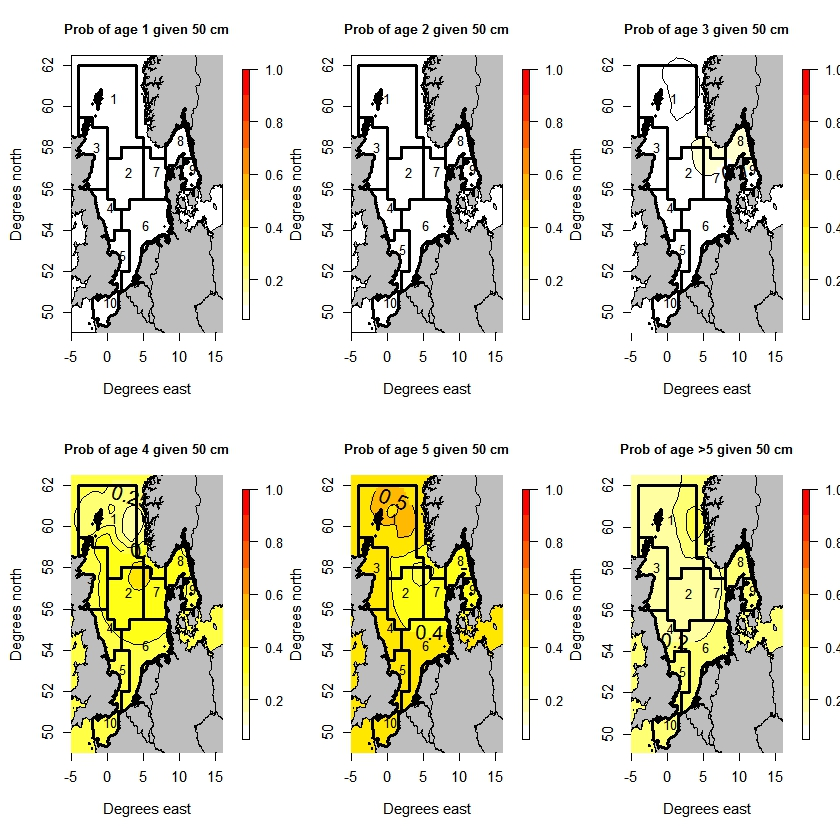
\includegraphics[width=15.5cm]{saithe2015Q1Map.jpeg}}   
% \captionsetup{font= footnotesize, width=15cm}{
% \caption{Estimated probability of age of a 50 cm long saithe in the first quarter of year 2015. The probability of age 1 to age 3 is approximately zero. The polygones marked 1 to 10 is the round fish areas (RFAs) where the ALK is assumed constant in the currently used estimators of the official CPUEs. The plots show that the age of saithe is more likely to be 5 given that it is 50 cm, particularly in RFA 1.}\label{saithe2015Q1Map}}
%\end{figure}



 
%\end{appendices}

\end{document}